\documentclass[master=elt,masteroption=im,english,oneside]{kulemt}
\newcommand*\classversion{1.8}
\newcommand*\manualdate{2015-06-01}
\setup{title={Writing a master thesis in LaTeX},
  subtitle={The `kulemt' v\classversion\ manual (\manualdate)},
  author={Luc Van Eycken},
  promotor={Prof.\,dr.\,ir. Y.~Berbers},
  assessor={Werkgroep masterproef},
  assistant={P. Wilson \and D. Knuth}}

%% Filing card information
\setup{filingcard,
  translatedtitle={Een masterproeftekst schrijven met LaTeX},
  udc=621.3,
  shortabstract={This document serves as the user manual for the
    \cls{kulemt} document class. The source of the class as well as the
    information for developpers is described in another document.
    \endgraf\smallskip
    This manual (dated \manualdate) describes the \cls{kulemt} class
    version~\classversion.}}

%% Fonts 
%  - Select the main text fonts: Utopia, Bera-Sans and LuxiMono
%    Remember their names, so we can use them in the text
\setup{font=utopia}
\newcommand*\rmfontname{Utopia}
\newcommand*\sffontname{Helvetica}
\newcommand*\ttfontname{Latin Modern Typewriter}
\IfFileExists{berasans.sty}{%
  \usepackage[scaled=.85]{berasans}%
  \renewcommand*\sffontname{Bera Sans}}{}
\IfFileExists{luximono.sty}{%
  \usepackage[scaled=.85]{luximono}%
  \renewcommand*\ttfontname{Luxi Mono}}{}

%% Additional formatting settings
%  - Use the chapter and headings styles as well as the ToC formatting
%    as defined in the kulemtx document style
\usepackage{kulemtx}
\headstyles{kulemtman}
\kulemtmanToC
%  - List are tighter than default
\firmlists
%  - Footnotes: set the marker flushleft and the text as a block paragraph
\setlength\footmarkwidth{1.5ex}
\setlength\footmarksep{0pt}
\footmarkstyle{\textsuperscript{#1}\hfill}
%  - Verbatim: I always use a tab setting of 8 characters
\tabson[8]
%  - URLs are always surrounded by angle brackets
%    Note: some PDF viewers require that URLs start with "http://"!
\usepackage{url}
\renewcommand*\UrlLeft{\langle\thinspace}
\renewcommand*\UrlRight{\thinspace\rangle}

%% Additional packages
%  - subfigures
\newsubfloat{figure}
%  - tikz/pgf
\usepackage{tikz}
\usetikzlibrary{arrows,calc}
%  - isodate (to properly print dates)
\usepackage[cleanlook,english]{isodate}

%% Finally hyperref is loaded for proper PDF links
%  Colors: external links in blue, internal ones in dark blue
\usepackage[pdfusetitle,colorlinks,
  filecolor={[rgb]{0,0,1}},urlcolor={[rgb]{0,0,1}},
  citecolor={[rgb]{0,0,.4}},linkcolor={[rgb]{0,0,.4}}]{hyperref}
\pdfstringdefDisableCommands{\let\cs\textbackslash}

%% Define some typesetting commands
%  NOTE: Please don't use logos (\LaTeX ...) in the text, but simply LaTeX ...
\newcommand*\acro[1]{{%
    \ifdim\csname f@size\endcsname pt<10pt\else \expandafter\small\fi #1}\@}
\newcommand*\cls[1]{\textsf{#1}}
\newcommand*\pkg[1]{\textsf{#1}}
\newcommand*\env[1]{\cmdprint{#1}}
\newcommand*\opt[1]{\texttt{#1}}
\newcommand*\file[1]{\texttt{#1}}
\newcommand*\PDF{\acro{PDF}}
\newcommand\Dutch[1]{`\foreignlanguage{dutch}{#1}'}
\newcommand\English[1]{`\foreignlanguage{english}{#1}'}
\newcommand*\NewInVersion[1]{\sidepar{\small\textcolor{gray}{New in v#1}}\ignorespaces}

\begin{document}

\begin{preface}
  I would like to thank everybody who has kept me busy with writing,
  debugging, and documenting this LaTeX document class. My thanks goes
  especially to my supervisor and my mentors. I also thank my assessors,
  at least those who read this text.

  Finally I would like to thank all the people who provided feedback,
  either with bug reports or by suggesting improvements.
\end{preface}

\tableofcontents*

\begin{abstract}
  This document describes the use of the LaTeX document class \cls{kulemt},
  which implements the KU~Leuven Faculty of Engineering guidelines for
  writing a master thesis. Since there are slight differences between the
  actual guidelines of the different engineering masters, this class
  implements not only the common part, but it also provides the necessary
  options to adapt it to the specific requirements. So please check the
  guidelines of your master before using or tweaking typesetting options.

  To illustrate the difference between the main text language and the
  master language, this document is written in English (as the main text
  language) for a Dutch master.

  This manual (dated \manualdate) describes the \cls{kulemt} class
  version~\classversion.
\end{abstract}

\begin{abstract*}
  Dit document beschrijft de LaTeX-documentklas \cls{kulemt}, die de
  richtlijnen van de Faculteit Ingenieurswetenschappen van de KU~Leuven
  voor het schrijven van een masterproeftekst implementeert. Maar vermits
  de richtlijnen van de verschillende ingenieursopleidingen licht
  verschillen, voorziet de documentklas de nodige opties om het resultaat
  aan te passen. Hou dus bij het aanmaken van de tekst niet zozeer rekening
  met wat de documentklas toelaat, maar wel met wat jouw master als
  specifieke richtlijnen opgeeft.

  Voor studenten van een Nederlandstalige master die hun masterproef in het
  Engels schrijven (bv.\ Erasmus-studenten) is een Nederlandse samenvatting
  verplicht. Als jouw master een uitgebreide samenvatting verlangt met
  figuren en tabellen kun je die best voorzien als een bijlage. Anders
  volstaat deze samenvatting van 1~bladzijde.

  Om het effect van twee talen te illustreren is dit document geschreven
  als een Engelse tekst (verder \English{text language} genoemd) voor een
  Nederlandstalige master (verder \English{master language} genoemd).

  Deze handleiding van \manualdate\ beschrijft de LaTeX-documentklas
  \cls{kulemt} versie~\classversion.
\end{abstract*}

\listoffiguresandtables

\mainmatter

\chapter{Writing a thesis in LaTeX}
A LaTeX document class has been developed, which follows the guidelines
described in \cite{kulemtgl}. The usage of this class is described in
\Cref{cha:kulemt}. The result can be customized and adapted to the masters'
guidelines with the class options. Additional functionality is available
through numerous LaTeX packages (cf.\ \Sref{sec:packages}). Just make sure
that the final result still conforms to the guidelines.

\Aref{app:template} contains a typical LaTeX template. Since each chapter
is a logical unit and since it's usually several pages long, chapters
should be put in independent files. They are called from the main file
using the LaTeX \cs{include} mechanism. The bibliography is a special case.
It is handled in \Sref{sec:bibtex}.

If you are not (yet) familiar with LaTeX, you should first have a look at the
documentation of the TeX Users Group on \url{http://tug.org/begin.html}.
It also contains a list of on-line tutorials and manuals. The most popular
(not so) short introduction to LaTeX is probably \cite{lshort}.
\Sref{sec:packages} contains some extra information on how to install LaTeX
packages. It also lists some typically useful packages.

\section{Using extra LaTeX packages}
\label{sec:packages}
Most of the packages mentioned in this document are present a standard
LaTeX installation, with the exception of the \pkg{kulemt} package. Apart
from this \pkg{kulemt} package, only a few packages are required. An
overview is given in \tref{tab:reqpack}.
\begin{table}[t]
  \caption[Packages used by \cls{kulemt} which may not be present in your
    LaTeX installation.]{Packages used by \cls{kulemt} which may not be
    present in your LaTeX installation. If a package is desirable but not
    required, it is used when available and ignored otherwise.}
  \label{tab:reqpack} 
  \centering
  \newcommand*\citepkg[1]{\pkg{#1}&\cite{pkg:#1}}
  \begin{tabular}{@{}l@{\space}ll@{}}
    \toprule
    Package           & & Remarks \\
    \midrule
    \citepkg{memoir}    & Required; at least version 1.61 (2004-04-05) \\
    \citepkg{microtype} & Desirable unless option \opt{nomicrotype} is used\\
    \pkg{lmodern} (\pkg{lm}) & \cite{pkg:lmodern}
                        & Desirable; required if \opt{font=lm} is used \\
    \citepkg{fourier}   & Only required if \opt{font=utopia} is used \\
    \bottomrule
  \end{tabular}
\end{table}

When you want to install a package, you can follow the instructions found
in the TeX-FAQ\,\cite{texfaq} under the heading ``Installing (La)TeX
files''. If you only can or want to install packages for your personal use,
make sure you read ``Private installations of files''.

The installation of the document class \cls{kulemt} is done in the same way
as the installation of any other package. The only difference is the fact
that its source is not available from \acro{CTAN} but from a local ftp
server\,\cite{pkg:kulemt}.

Apart from the required packages, a lot of packages are available from
\acro{CTAN}\,\cite{CTAN}\footnote{An alphabetic and a topical index is
  provided by the TeX Catalogue\,\cite{texcatalogue}.}, which can help you
to make your text easier to understand or more impressive. Many of them are
installed by default in a traditional LaTeX installation. Some typical
examples are given in \tref{tab:otherpack}.
\begin{table}
  \caption{Packages which can be useful to extend the \cls{kulemt} class.}
  \label{tab:otherpack}
  \centering
  \renewcommand*\thefootnote{\fnsymbol{footnote}}
  \begin{tabular}{@{}ll@{}}
    \toprule
    Package        & Description \\
    \midrule
    \pkg{hyperref} & Provide hyperlinks in \PDF\ files \\
    \pkg{amsmath}  & Extra mathematical constructs \\
    \pkg{amssymb}  & Extra mathematical symbols\footnotemark[1]
                         (only for the fonts \opt{cm} \& \opt{lm}) \\
    \pkg{cite}     & Better references \\
    \pkg{babelbib} & Multilingual or non-English bibliographies \\
    \pkg{flafter}\footnotemark[2]
                   & Put figures \& tables always after their definition \\
    \pkg{rotating} & Rotating material, e.g., figures en tables \\
    \pkg{listings} & Typeset programming code \\
    \pkg{nomencl}  & Produce lists of symbols (nomenclature) \\
    \pkg{pgf}      & Create graphics in LaTeX \\
    \pkg{siunitx}  & Consistent use of SI units \\
    \pkg{textcomp}\footnotemark[2]
                   & Extra text symbols\footnotemark[1]
                         (e.g., \cs{texteuro} = \texteuro)\\
    \bottomrule \addlinespace
    \multicolumn2{l}{\footnotemark[1] \footnotesize
      A list of all kind of symbols is found in \cite{symbols}.} \\
    \multicolumn2{l}{\footnotemark[2] \footnotesize
      Information on this package is found in the TeX-FAQ\,\cite{texfaq}.} \\
  \end{tabular}
\end{table}
The loading order can be important for some combination of packages:
packages, which extend or redefine commands of other packages, must be
loaded last.

If you are making a \PDF\ file for on-line distribution, the use of the
\pkg{hyperref} package\,\cite{pkg:hyperref} is a must. It not only
automatically generates the bookmarks, but it also gives you all the
linking facilities required in modern on-line documents\,\footnote{This
  document uses as \pkg{hyperref} options: ``\opt{pdfusetitle,
    colorlinks, \let\meta\relax filecolor=\marg{\oarg{rgb}\marg{0,0,1}},
    urlcolor=\marg{\oarg{rgb}\marg{0,0,1}},
    citecolor=\marg{\oarg{rgb}\marg{0,0,0.4}},
    linkcolor=\marg{\oarg{rgb}\marg{0,0,0.4}}}''.}.

The \pkg{microtype} package\,\cite{pkg:microtype} enhances the typographic
quality of the text. Therefore the \cls{kulemt} class uses it by default.
The most important enhancements provided by the package are character
protrusion and font expansion. Character protrusion lets some characters
enter the margin to provide optical margins. Font expansion creates fonts
which are a little bit narrower or wider. It generates more equal interword
spacing and it provides also more flexibility to avoid hyphenation. Both
effects are illustrated in \fref{fig:microtype}.
\begin{figure}
  \centering
  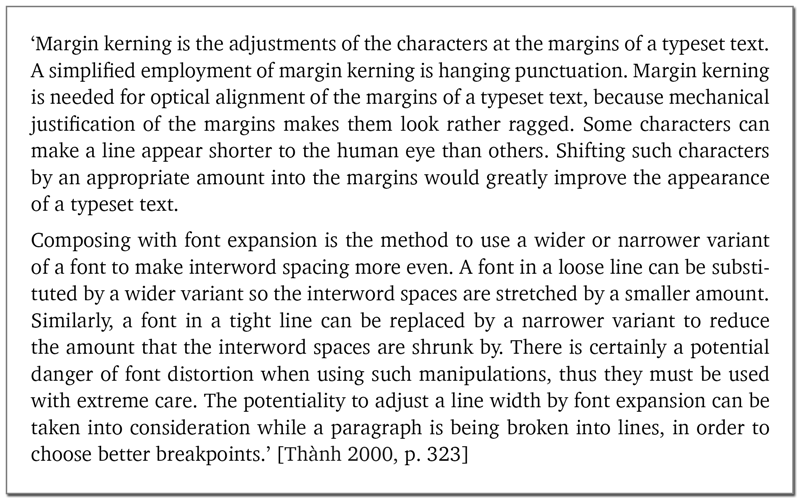
\includegraphics[width=\columnwidth]{expfprof.png}%
  \subcaption{Text typeset without using \pkg{microtype}.}
  \par\bigskip
  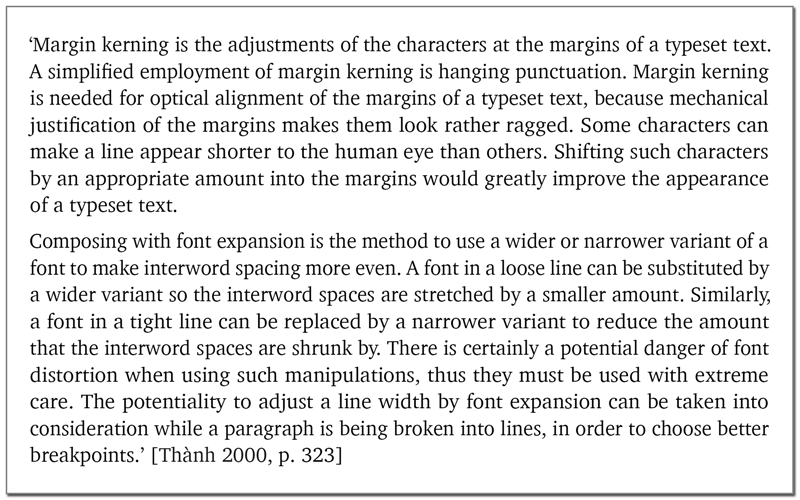
\includegraphics[width=\columnwidth]{exptprot.png}%
  \subcaption{The same text typeset using \pkg{microtype} (character
    protrusion \& font expansion).}
  \caption[The effect of using the \pkg{microtype} package.]{The effect of
    using the \pkg{microtype} package. These examples are borrowed from the
    \pkg{microtype} manual.}
  \label{fig:microtype}
\end{figure}

%\enlargethispage{3pt}
The document class \cls{memoir} includes or emulates a lot of packages. The
exact list of packages included or emulated in \cls{memoir} can always be
found in the log file after a LaTeX run. The emulation not always
corresponds to the latest version of the package, but the main
functionality is usually present. So before installing a new package, first
check the \cls{memoir} manual to see if the functionality is not already
present in the document class.

Since the document class \cls{kulemt} is based on \cls{memoir} it also
includes all packages included or emulated by \cls{memoir\,\footnote{The
    \cls{memoir} class dated 2005-09-25 emulates the packages
    \pkg{abstract}, \pkg{appendix}, \pkg{array}, \pkg{booktabs},
    \pkg{ccaption}, \pkg{chngcntr}, \pkg{chngpage}, \pkg{crop},
    \pkg{dcolumn}, \pkg{delarray}, \pkg{enumerate}, \pkg{epigraph},
    \pkg{framed}, \pkg{ifmtarg}, \pkg{ifpdf}, \pkg{index}, \pkg{makeidx},
    \pkg{moreverb}, \pkg{needspace}, \pkg{newfile}, \pkg{nextpage},
    \pkg{patchcmd}, \pkg{shortvrb}, \pkg{showidx}, \pkg{tabularx},
    \pkg{titleref}, \pkg{titling}, \pkg{tocbibind}, \pkg{tocloft},
    \pkg{verbatim}, and \pkg{verse}. The version dated 2009-11-17 adds the
    packages \pkg{changepage}, \pkg{ifetex}, \pkg{ifluatex}, \pkg{ifxetex},
    \pkg{mparhack}, \pkg{pagenote}, \pkg{parskip}, and \pkg{setspace}.}}.
It further includes some standard packages (\pkg{babel}, \pkg{color},
\pkg{graphicx}, and \pkg{keyval}) as well as the packages mentioned in
\tref{tab:reqpack}.

\section{Using BibTeX for the bibliography}
\label{sec:bibtex}
The bibliography can be input as a list in the text, using the
\env{thebibliography} environment. An alternative way to generate a
bibliography is with the help of the BibTeX program, which is always
included in a LaTeX distribution. More information on building a
bibliography can be found in \cite{tamethebeast} and \cite{btxfaq}.

The bibliographic data is stored in one or more bibliographic files (files
with extension ``\file{.bib}''). For some disciplines existing data files
can be used. They are declared with the \cs{bibliography} command. A
personal data file can also be used \cite[part~3]{tamethebeast}. It's no
problem if the data files contain unneeded items because only the
referenced items will be used.

The actual layout and formatting is determined by the bibliography style.
This style is declared by the \cs{bibliographystyle} command, which refers
to a file with extension ``\file{.bst}''. The master guidelines or the
thesis supervisor determine which bibliography style to use. If none is
specified, you can choose whichever you find most suited for your text.

Some bibliography styles needs additional LaTeX commands for proper
operation. These commands are defined in an accompanying LaTeX style file,
which must be required with \cs{usepackage}. An example is
\pkg{IEEEtrantools}, which defines the command \cs{bstctlcite} to control
the parameters of the \pkg{IEEEtran} bibliography style\footnote{Both the
  \pkg{IEEEtran} bibliography style and the \pkg{IEEEtrantools} style file
  are part of the \pkg{IEEEtran} package\,\cite{pkg:IEEEtran}.}, which is
used in this document. This bibliography style can be used to typeset a
bibliography according to the rules of IEEE\@.

LaTeX packages can also be used to change the formatting of the citations
in text. A popular one is the \pkg{natbib} package \cite{pkg:natbib}. It is
compatible with many bibliography styles and it allows both author-year and
numerical citations.

\section{Using \file{latex} or \file{pdflatex}?}
\label{sec:engine}

The ways to compile a LaTeX file are shown in \fref{fig:compile}.
\begin{figure}
  \newcommand*\pnode[2][]{\path (#2) node[rectangle, draw, thick,
    minimum width=20\unitlength, minimum height=10\unitlength,#1]}
  \newcommand*\fnode[2][]{%
    \draw[thick,#1] (#2) +(-5,5) -- +(5,5) --
      +(5,-5) .. controls +(3,-3)  and +(2,1)  .. % (-2,2)  & (2,1)
      +(0,-5) .. controls +(-2,-6) and +(2,-2) .. % (-2,-1) & (2,-2)
      +(-5,-5) -- cycle;
    \path (#2) node[rectangle, minimum width=10\unitlength,
                    minimum height=10\unitlength]}
  \setlength\unitlength{1mm}
  \centering
  \begin{tikzpicture}[x=\unitlength, y=\unitlength, semithick, >=stealth']
    \ttfamily\small
    %% program nodes
    \pnode{30,17}(pltx){latex};
    \pnode[dashed]{80,10}(pbtx){bibtex};
    \pnode{80,25}(pdps){dvips};
    \pnode[dotted]{80,40}(pp2p){ps2pdf};
    %% file nodes
    \fnode{  5,25}(ftex){.tex};
    \fnode{ 55,25}(fdvi){.dvi};
    \fnode{102,25}(fps){.ps};
    \fnode{ 55,10}(faux){.aux};
    \fnode[dashed]{102,10}(fbbl){.bbl};
    \fnode[dotted]{102,40}(fpdf){.pdf};
    %% arrows
    \draw[->] (ftex.east) -- ++(5,0) |- ($(pltx.west)+(0,2.5)$);
    \draw[->] ($(pltx.east)+(0,2)$)  -- ++(5,0) |- (fdvi.west);
    \draw[->] (fdvi) -- (pdps);
    \draw[->] (pdps) -- (fps);
    \draw[->] ($(pltx.east)+(0,-2)$) -- ++(5,0) |- (faux.west);
    \draw[->] (faux.east) -- ++(4,0) |- (15,2)
              |- ($(pltx.west)+(0,-2.5)$);
    \draw[dashed,->] ($(faux.east)+(4,0)$)  -- (pbtx);
    \draw[dashed,->] (pbtx) -- (fbbl);
    \draw[dashed,->] (fbbl.east) -- ++(5,0) |- (12,0) |- (pltx.west);
    \draw[dotted,->] (fps.east) -- ++(5,0) |- (65,32) |- (pp2p.west);
    \draw[dotted,->] (pp2p) -- (fpdf);
  \end{tikzpicture}\medskip
  \subcaption{Converting a LaTeX file to PostScript (or \PDF\ with the dotted
    part added) using \file{latex}.\label{fig:latex}}
  \par\bigskip\bigskip
  \begin{tikzpicture}[x=\unitlength, y=\unitlength, semithick, >=stealth']
    \ttfamily\small
    %% program nodes
    \pnode{30,17}(pltx){pdflatex};
    \pnode[dashed]{80,10}(pbtx){bibtex};
    %% file nodes
    \fnode{ 5,25}(ftex){.tex};
    \fnode{55,25}(fpdf){.pdf};
    \fnode{55,10}(faux){.aux};
    \fnode[dashed]{102,10}(fbbl){.bbl};
    %% arrows
    \draw[->] (ftex.east) -- ++(5,0) |- ($(pltx.west)+(0,2.5)$);
    \draw[->] ($(pltx.east)+(0,2)$)  -- ++(5,0) |- (fpdf.west);
    \draw[->] ($(pltx.east)+(0,-2)$) -- ++(5,0) |- (faux.west);
    \draw[->] (faux.east) -- ++(4,0) |- (15,2)
              |- ($(pltx.west)+(0,-2.5)$);
    \draw[dashed,->] ($(faux.east)+(4,0)$)  -- (pbtx);
    \draw[dashed,->] (pbtx) -- (fbbl);
    \draw[dashed,->] (fbbl.east) -- ++(5,0) |- (12,0) |- (pltx.west);
  \end{tikzpicture}\medskip
  \subcaption{Converting a LaTeX file to \PDF\ using \file{pdflatex}.%
    \label{fig:pdflatex}}
  \par\medskip
  \caption[Steps to compile a LaTeX file]{Steps to compile a LaTeX file.
    The dashed part is needed only if a BibTeX bibliography is used.
    As long as the \file{.aux} file (or the \file{.bbl} file) changes,
    (\file{pdf})\file{latex} must be invoked.}\label{fig:compile}
\end{figure}
The traditional way uses the \file{latex} program (\fref{fig:latex}). It
outputs the typeset document to a \file{.dvi} file, which is rather TeX
specific. So usually this is converted to a PostScript file using
\file{dvips} or a \PDF\ file using \file{dvips}~+~\file{ps2pdf} or
\file{dvipdfm}.

Several iterations of \file{latex} may be required. Each time the contents
of an auxiliary file (such as \file{.aux} or \file{.bbl}) changes,
\file{latex} must be invoked. This often means three iterations. The first
invocation of \file{latex} generates a list of internal references and of
referenced bibliography items in the \file{.aux} file. The latter is used
by \file{bibtex} to produce the bibliography data in the \file{.bbl} file.
A second iteration uses the bibliography data and the values from the
references from the \file{.aux} file to generate the final content
containing the table of contents and the bibliography. Because this may
introduce new content, labelled items may shift. This requires an additional
iteration of \file{latex} to get the changed references right. The exact
number  of iterations depends on how much references change from one
version of the \file{.tex} file to the next version. If you use an
intelligent editor, such as Emacs with AUCTeX, you needn't guess
yourself: the editor will tell you when an extra iteration is needed.

If you want a \PDF\ file as a result\,\footnote{Every master thesis must
  also be submitted electronically in \PDF!}, it's easier to use
\file{pdflatex} than \file{latex}, as illustrated in \fref{fig:pdflatex}.
But \file{pdflatex} has other advantages too. It uses the pdfTeX engine,
which is an enhanced implementation of the TeX engine used by \file{latex}.
Therefore more advanced features, such as breaking hyperlinks
(\pkg{hyperref} package) or font expansion (\pkg{microtype} package), are
only possible with the pdfTeX engine. Additionally, the pdfTeX engine can
directly include images in the \acro{JPEG} or \acro{PNG} file format as
well as other \PDF\ files. Simple PostScript (e.g., as generated by
MetaPost) can also be included but general \acro{EPS} (Encapsulated
Postscript) not. You'll have to convert the latter to \PDF\ with the
\file{epstopdf} program.

Is there any reason to use \file{latex}? The most important reason is the
fact that your text depends on packages which work only with PostScript
output, such as \pkg{psfrag} or all kind of PSTricks packages. But often
valid or even better replacements exist, such as the \pkg{pgf}
package\,\cite{pkg:pgf}. Conversion tools may also be available (e.g., the
\pkg{pst-pdf} package).
Another valid reason to stick to \file{latex} is the fact that your
thesis supervisor wants you to use it. In this case I hope you can educate
him/her to upgrade to a newer way of working.

You even have more choices than \file{latex} and \file{pdflatex}. A modern
installation also provides \file{xelatex} and \file{lualatex}. Unless you
know what you're doing, I wouldn't recommend them. Furthermore the LaTeX
document class \cls{kulemt} has never been tested with one of them. So it's
very likely you run into problems if you use them.

A final word of advice: don't switch between engines gratuitously. To avoid
errors and text drifting to other places, always use either \file{latex} or
\file{pdflatex}.


%%% Local Variables: 
%%% mode: latex
%%% TeX-master: "kulemt"
%%% End: 

\newcommand*\optionlabel[1]{\hspace\labelsep
  \let\oldmeta\meta \renewcommand*\meta[1]{{\rmfamily \oldmeta{##1}}}%
  \renewcommand*\and{\unskip\textrm{'' or ``}}%
  \normalfont \textsc{Option%
    \csname kulemt@ifand\endcsname{#1}s} ``\opt{#1}''}
\newcommand*\optionlabelnote[1]{\hfill \textit{(#1)}}
\newcommand*\betweenarrows[1]{%
  $\leftarrow\mkern-7mu\cleaders\hbox{$\mkern-2mu\relbar\mkern-2mu$}\hfill
   \enspace\hbox{#1}\enspace
   \cleaders\hbox{$\mkern-2mu\relbar\mkern-2mu$}\hfill\mkern-7mu\rightarrow$}

\chapter{The LaTeX document class \cls{kulemt}}
\label{cha:kulemt}
The document class \cls{kulemt} can be used to generate a master thesis
text which is conform to the guidelines of the KU~Leuven Faculty of
Engineering. It is actually an extension of the \cls{memoir} document
class\,\cite{pkg:memoir}, which already includes the functionality of the
most useful LaTeX packages. So before starting to use the \cls{kulemt}
document class, you should read the \cls{memoir} manual\,\cite{memman} first!

The default styling of the chapter and section headings is pretty plain. Of
course you can tweak all parameters yourself, but the \cls{memoir} class
provides consistent alternatives using the \cs{headstyles}
command\,\cite[\S6.9]{memman}. For changing only the chapter heading style,
the \cs{chapterstyle} command\,\cite[\S6.5]{memman} is available. The
chapter and headings style used by this document are available in the
\pkg{kulemtx} document style, which is part of the \cls{kulemt} package.
More examples of chapter styles are available from \cite{memchap}.

By default, the \cls{kulemt} class tries to load the \pkg{microtype}
package, because this package contributes to the typographic quality of the
text, as illustrated in \fref{fig:microtype}. It gives us less hyphenation
(thanks to the use of font expansion) and optical alignment (thanks to
character protrusion). Since this package only works properly with
\file{pdflatex} in \PDF\ mode, it's only loaded by default in this mode.
The option \opt{nomicrotype} (cf.\ page~\pageref{opt:nomicrotype}) cancels
the loading of the package.

\section{Options}\label{sec:options}
The document class can be customized by the user through options. The
options come in three flavors. A first set of options, called
\emph{document class options}, can only be used as options of the
\cs{documentclass} command. They are processed in the order of appearance.
The reason for having document class options is that an option is needed as
a global option, which can also be used by other packages, or that an
option is used during the initialization of the class itself. The other
options can be used everywhere in the document preamble, either as
option of \cs{documentclass} or as an argument of a \cs{setup} command. But
some of these options, called \emph{once-only options}, can only be given
once. The remaining options, called \emph{unrestricted options}, can be
used multiple times.

Many options are specified as ``\meta{key}\texttt{=}\meta{value}''. If the
value contains a comma or a space, it must be enclosed in braces:
``\meta{key}\texttt{=}\marg{value}''. Due to the implementation of LaTeX2,
options of the \cs{documentclass} can't contain commands or spaces,
contrary to the argument of \cs{setup}\label{com:setup}. Therefore it's
better to put all options, except the document class options, in the
argument of one or more \cs{setup} commands. The document preamble can
contain multiple \cs{setup}\marg{optionlist} commands. The
\meta{optionlist} is a comma separated list of options. If unrestricted or
document class options are given multiple times, usually the last value
survives unless mentioned otherwise (e.g., the \opt{extralanguage} option).

\subsection{Selecting the master}
\begin{labelled}{optionlabel}
\item[master=\meta{id\,}]\optionlabelnote{required document class option}\\
  The supported master \meta{id\,}s are defined in the configuration file.
  The currently supported \meta{id\,}s for the Faculty of Engineering are
  enumerated in \Sref{sec:mastercfg}.

  The \opt{master} option is used to indicate the master degree this
  thesis is written for. Only one \opt{master} option can be given in
  the document, which makes it impossible to generate one text for
  different masters, even if it is a common work of two or more students
  from different masters. This scenario was considered too unlikely to
  support, also because each master may have its own additional
  requirements on content and layout.

  \NewInVersion{1.4}
  Obsolete master definitions may still be available for printing older
  material. See \Sref{sec:obsoletemasters} for available obsolete masters.
  Note that an \meta{id\,} may change when it becomes obsolete to avoid
  conflicts with valid \meta{id\,}s.

\item[masteroption=\meta{mo}]\optionlabelnote{once-only option}\\
  This option specifies the master option (\Dutch{optie}) or the major
  topic (\Dutch{afstudeerrichting}) of the master degree. The value
  \meta{mo} is either an abbreviation or a text describing the master
  option. The known master option abbreviations are also defined in the
  configuration file. The currently supported master option abbreviations
  for the Faculty of Engineering are enumerated in \Sref{sec:mastercfg}. If
  a text is used for \meta{mo}, it must start with the appropriate word in
  lower case: ``\texttt{option }\ldots''
  (``\texttt{\foreignlanguage{dutch}{optie} }\ldots'' or
  ``\texttt{\foreignlanguage{dutch}{afstudeerrichting} }\ldots'' in Dutch).
  Examples of full text can be found in \Sref{sec:mastercfg}. As mentioned
  above, if \meta{mo} contains spaces, you can't use this as a document
  class option.

  Whether or not a master option must be specified depends on your master
  guidelines. Some masters even don't allow you to print a master option on
  the front pages. You can find all this information also in
  \Sref{sec:mastercfg}.
  \NewInVersion{1.7}%
  An error is raised if the master requires you to specify a master option
  and \opt{masteroption} is not used. An error is also raised if you use
  \opt{masteroption} and your master disallows master options.

  If a group of students from different master options produces a single
  text, the \meta{mo} can be replaced by a comma separated list of
  \meta{mo}s. Each of these list elements can either be an abbreviation or
  a full text. 

  \NewInVersion{1.6}
  Obsolete master options may still be available for printing older
  material. Available obsolete options are also listed in
  \Sref{sec:mastercfg}. Note that abbreviations may change when they become
  obsolete to avoid conflicts with valid options.
\end{labelled}

\subsection{Declaring the language(s)}
The commands of the \pkg{babel} package can be used to select a language.
Currently only Dutch and English are supported as text language, but other
languages can be used for short fragments of text. The master language is
defined by the master degree itself, so it can't be chosen.

Whatever language you choose, some parts are always in Dutch and some parts
always in English. Since these two language must be available, an error is
raised if their hyphenation patterns are not preloaded in your installation.

\begin{labelled}{optionlabel}
\item[dutch \and english]\optionlabelnote{document class options}\\
  These options select the text language, either Dutch or English.
  Both options are mutually exclusive: at most one of the options can be used.
  If none of the options is used, the text language is Dutch.

  Since these options are document class options, they are global LaTeX
  options. This means that other packages which are language sensitive will
  also use these options.

\item[extralanguage=\meta{lang}]\optionlabelnote{document class option}\\
  To switch the language of text fragments commands such as
  \cs{foreignlanguage} from the \pkg{babel} package. But only languages
  which have been defined can be used. By default only English and Dutch
  are defined. If other languages are needed, they must be declared with
  this \opt{extralanguage} option. The \meta{lang} can be any language
  known to \pkg{babel}.

  If multiple languages must be declared you have to use this option
  several times. This is one of the options where values accumulate instead
  of overwrite each other.
\end{labelled}

\subsection{Information for the title page}
These options provide the necessary information for the title page and the
cover page. Since either of these pages must be present, most of the
options are required.

\begin{labelled}{optionlabel}
\item[title=\meta{title}]\optionlabelnote{required unrestricted option}\\
  This option provides the official title \meta{title} of the thesis. It
  must be written in the text language, which may be different from the
  master language.

\item[subtitle=\meta{stitle}]\optionlabelnote{unrestricted option}\\
  A subtitle \meta{stitle} is optional. It is only used on the cover and
  the title page. It will not be used in any bibliographic reference.

\item[author=\meta{authors}]
  \optionlabelnote{required unrestricted option}\label{opt:author}\\
  This option provides the name \meta{authors} of the author(s) of the
  thesis. The name consists of a non-abbreviated first name followed by the
  last name without a comma in between. If the thesis text has multiple
  authors, they are all listed in \meta{authors}, separated by a command
  \cs{and}.

\item[promotor=\meta{promoters}]
  \optionlabelnote{required unrestricted option}\\
  This option lists the \meta{promoters} (a.k.a.\ thesis supervisors). If
  the thesis has multiple supervisors and/or co-supervisors, they are all
  listed in \meta{promoters}, separated by a command \cs{and}. The name of
  each supervisor is preceded by his/her title unless stated otherwise in
  the master guidelines.

  The \meta{promoters} value also lists the co-supervisors. Co-supervisors are
  always given after the supervisor(s). Nothing is provided to differentiate
  between supervisors and co-supervisors. However your master may have
  additional guidelines about this.

\item[promoter=\meta{promoters}]
  \NewInVersion{1.7}\\
  This option is an alias for the option ``\opt{promotor}''.

\item[assessor=\meta{assessors}]
  \optionlabelnote{required unrestricted option}\\
  This option lists the \meta{assessors} of the thesis separated by a
  command \cs{and}. The name of each assessor is preceded by his/her
  title unless stated otherwise in the master guidelines. For assessors
  from other universities or companies, their affiliation can be mentioned
  if the master guidelines require it.

  \NewInVersion{1.2} If you don't have any assessor, contrary to the
  faculty rules, you must use this required option but with an empty value
  for \meta{assessors}, e.g., use ``\verb"assessor="'' as an option.

\item[assistant=\meta{assistants}]
  \optionlabelnote{required unrestricted option}\\
  This option lists the \meta{assistants} (a.k.a.\ mentors) of the thesis
  separated by a command \cs{and}. For mentors from other universities
  or companies, their affiliation can be mentioned if the master guidelines
  require it.

  \NewInVersion{1.2} If you worked without the help of a mentor, you can
  use this required option with an empty value for \meta{assistants}, e.g.,
  use ``\verb"assistant="'' as an option.

\item[acyear=\meta{acyear}]\optionlabelnote{unrestricted option}\\
  This option sets the academic year the master degree is obtained. The
  \meta{acyear} should have a format like ``\verb*"{2009 -- 2010}"''.

  The default is the current academic year. If the \file{latex} run is
  after October 1, the current year defines the start of the academic year.
  Otherwise it defines the end of the academic year. So this option should
  probably only be used in case of emergency because the default works quite
  well.
\end{labelled}

\subsection{Additional information for the filing card}
Some masters require a filing card (known in Dutch as a
`\foreignlanguage{dutch}{fiche}') either in the text itself or to be
printed on a separate page\,\footnote{The option \opt{frontpagesonly}
  can be used to print the filing card.}. This also means that the required
options in this section are only required if a filing card is used. 
\begin{labelled}{optionlabel}
\item[translatedtitle=\meta{title2\,}]
  \optionlabelnote{required unrestricted option}\\
  The faculty requires a translated title \meta{title2\,} for Dutch
  masters: in English when the thesis is written in Dutch, and in English
  otherwise. A thesis in English of an English master doesn't need a
  translated title. In this case \meta{title2\,} should be set to an empty
  value (cf.\ \Sref{sec:file:main}).

\item[shortabstract=\meta{short abstract}]
  \optionlabelnote{required unrestricted option}\\
  The filing card also contains a short abstract, which should be no longer
  than 500~words. This option specifies the \meta{short abstract}. The
  language of this abstract is the same as the main text language.

  Any LaTeX command or environment can be used in this \meta{short
    abstract} except the \cs{par} command. Since a blank line corresponds
  to a \cs{par} command, blank lines can't be used either. If you want to
  start a new paragraph, you have to use the \cs{endgraf} command instead.

\item[udc=\meta{UDC nr}]\optionlabelnote{required unrestricted option}\\
  The\meta{UDC nr} can be obtained either from your master secretary or
  from the library. Please consult your master secretary first.

\item[keywords=\meta{keywordlist}]\optionlabelnote{unrestricted option}\\
  A list of keywords can be added with this option. The \meta{keywordlist}
  is a comma separated list of keywords with a space after each comma.

  Some masters require this option to be used. Since the typically used
  keywords depend on the discipline, consult your thesis supervisor for
  suggestions if you are using this option.

\item[articletitle=\meta{arttitle}]\optionlabelnote{unrestricted option}\\
  Some masters require an additional article either to be included in the
  thesis text or to be provided separately. This optional option provides
  the title \meta{arttitle} of the article for printing on the filing card.
\end{labelled}

\subsection{Conditionally generating pages}
The options in this section determine which pages are available in the
output file.

\begin{labelled}{optionlabel}
\item[coverpageonly]\optionlabelnote{unrestricted option}\\
  If this option is used, only the cover page is printed. This option
  supersedes any other option from this section.

\item[frontpagesonly]\optionlabelnote{unrestricted option}\\
  If this option is used, only the front pages are printed instead of the
  entire document. The front pages include the title page, the copyright
  page and the filing card (if wanted). You can use this option to generate
  these pages when you are using other text processing software to write
  your thesis.

\item[filingcard]\optionlabelnote{unrestricted option}\\
  By default no filing card is included in the text unless the master is
  known to require one. With this option you can force the inclusion of a
  filing card in your text.
\end{labelled}

\subsection{The layout of the typeblock}
These options customize the layout of the text area on the page. Most of
them are options available to all traditional LaTeX document classes.

\begin{labelled}{optionlabel}
\item[10pt \and 11pt]\optionlabelnote{document class options}\\
  The default font size of the main text can be set to 10\,pt or 11\,pt.
  The options are mutually exclusive. The default size is 11\,pt.

  All other fonts used in the text are scaled proportionally. Additionally
  the line width of a 10\,pt text is decreased by 1\,cm because of
  readability reasons.

\item[oneside \and twoside]\optionlabelnote{document class options}\\
  These mutually exclusive options declare whether the document will be
  printed on both sides of the paper or only on one side. The default value
  is \opt{twoside}.

  The \opt{twoside} option indicates that the text will be printed on both
  sides of the paper. The \opt{oneside} option indicates that it either
  will be printed on one side or it will be available for on-screen viewing
  only.

  The \cls{kulemt} document class has been designed to guarantee that the
  only thing which changes, when changing between \opt{oneside} and
  \opt{twoside}, is the horizontal position of the typeblock and eventually
  the locations of margin paragraphs. This means that you can without
  problems use the \opt{twoside} option to generate the printed version and
  the \opt{oneside} option for the \PDF\ version.

\item[openright \and openleft \and openany]
  \optionlabelnote{document class options}\\
  These options determine the page on which a new chapter in the main
  matter starts:
  \begin{itemize}
  \item \opt{openright}: Each main matter chapter starts on a recto page.
  \item \opt{openleft}: Each main matter chapter starts on a verso page.
  \item \opt{openany}: A main matter chapter can start on any page.
  \end{itemize}

  The three options are mutually exclusive. The default value is
  \opt{openright}. For one-side printing only recto pages are used, so
  these options are irrelevant.

  The \cls{memoir} class also provides the \cs{openright}, \cs{openleft},
  and \cs{openany} commands to change this inside the document itself.

\item[bind=\meta{binding length}]\optionlabelnote{document class option}\\
  When you open a two-side printed book, some paper of the inner margins is
  invisible due to the binding of the book. It seams as if the inner
  margins are smaller than specified. This option specifies the amount
  \meta{binding length} of the invisible inner margin of a page. This amount
  is specified as a length (e.g., \opt{3mm}) and it defaults to
  0\,mm.


\item[bindcover=\meta{binding tape width}]%
  \optionlabelnote{unrestricted option}%
  \NewInVersion{1.6}\\
  % When you are using a tape to bind your thesis, the tape may overlap with
  % the left logo on the cover page. This option specifies the amount
  % \meta{binding tape width} which covers the left margin on the cover page.
  % If this exceeds the available margin, the text width of the cover page is
  % reduced accordingly. The option has only effect on the cover page and it
  % is independent of the \opt{bind} option. Because of the cover page
  % layout, the maximum allowed \meta{binding tape width} is 25\,mm.
  \NewInVersion{1.7}
  Because of the new layout of the cover page, this option has become
  obsolete. So it has no effect.
\end{labelled}

\subsection{The text encoding}
The text encoding specifies the character encoding of the input files. By
default a pure {\small ASCII} encoding is expected.

\begin{labelled}{optionlabel}
\item[inputenc=\meta{enc}]\optionlabelnote{once-only option}\\
  This option lets you select another encoding of the input files using the
  \pkg{inputenc} package. As a value of \meta{enc} any option of the
  \pkg{inputenc} package is allowed. Typical examples are `\opt{latin1}'
  for ISO Latin-1 encoding (aka ISO-8859-1 encoding) or `\opt{utf8}' for
  UTF-8 encoding. See the documentation of the \pkg{inputenc} package for
  more information. When some LaTeX packages are installed on your system,
  they define additional encodings, e.g., the extended UTF-8 encoding
  `\opt{utf8x}' is installed by the \pkg{ucs} package.

  \NewInVersion{1.7}
  The \pkg{inputenc} package is initially loaded with its \opt{ascii}
  option. This helps you to detect a missing \opt{inputenc} option in your
  source file, since it will result in an error message such as
\begin{verbatim}
  ! Package inputenc Error: Keyboard character used is undefined
  (inputenc)                in inputencoding `ascii'.
\end{verbatim}
\end{labelled}

\subsection{Selecting fonts}
The guidelines only give some general hints about fonts, but they don't
enforce specific fonts. The following options predefine some font
combinations which are available in most LaTeX distributions. But you don't
have to choose one of them; you can select your own combination of fonts
using standard LaTeX packages. If no fonts are defined, either with the
options below or with LaTeX packages, the default LaTeX fonts (Computer
Modern) are used.

A font encoding tells LaTeX how to print a character with a
font\,\cite{encguide}. E.g., `\ss' is character 25 of font \file{cmr}
(\textsf{OT1} encoding) but it is character 255 of font \file{lmr}
(\textsf{T1} encoding). Modern LaTeX fonts can best be used with the newer
\textsf{T1} encoding; some of them are even not available in the old default
\textsf{OT1} encoding.

\begin{labelled}{optionlabel}
\item[font=\meta{fnt}\textrm{'' or ``}font=\meta{fnt}:\meta{fntopts}]
  \optionlabelnote{once-only option}\\
  This option chooses a predefined font family \meta{fnt}. The allowed
  values of \meta{fnt} are given in \tref{tab:fonts}\@, which shows the
  most important characteristics of the font families. For each family
  three related typefaces are defined: a serif typeface for normal text and
  math, a sans-serif typeface and a fixed-width typeface. If possible the
  \textsf{T1} font encoding is used. Some of these font families may require
  additional packages to be installed as indicated in \tref{tab:reqpack}.
  \begin{table}
    \caption[Predefined font families.]{Predefined font families. The default
      one is \opt{cm}.}\label{tab:fonts}
    \centering
    \renewcommand*\thefootnote{\fnsymbol{footnote}}
    \begin{tabular}{@{}>{\ttfamily}cccccc@{}}
      \toprule
      \opt{\meta{fnt}}
               & \multicolumn{4}{c}{typefaces} & \opt{\meta{fntopt}} = \\
      \cmidrule{2-5}
               & serif   & sans    & fixed width & math     & options from \\
      \midrule
      cm\,\footnotemark[1]
               & \multicolumn{4}{c}{\betweenarrows{Computer Modern}} & --- \\
      lm       & \multicolumn{4}{c}{\betweenarrows{Latin Modern}}    & --- \\
      palatino & Palatino&Helvetica&Latin Modern & Palatino & \pkg{mathpazo}\\
      times    & Times   &Helvetica&Latin Modern & Times\,\footnotemark[2]
                                                            & \pkg{mathptmx}\\
      utopia   & Utopia  &Helvetica&Latin Modern & Utopia   & \pkg{fourier} \\
      \bottomrule \addlinespace
      \multicolumn{6}{l}{\footnotemark[1] \footnotesize
        This family uses the old \textsf{OT1} font encoding instead of the
        new \textsf{T1} encoding.}\\
      \multicolumn{6}{l}{\footnotemark[2] \footnotesize
        No math version `\texttt{boldmath}' available.}\\
    \end{tabular}
  \end{table}

  Finding a matching math font is often a problem. Math fonts are available
  for all predefined fonts, although Times lacks a \texttt{boldmath}
  version. Often additional symbols are available for specific math fonts.
  For more information take a look at the documentation of the package,
  which loads the math fonts. The name of this math package is given in the
  last column of \tref{tab:fonts}. The second format of the \opt{font}
  option lets you specify additional options \meta{fntopts} for the math
  package.

  The default font family is \opt{cm} (in \textsf{OT1} encoding), because
  this is the LaTeX default.
\end{labelled}


\subsection{Other options}
\begin{labelled}{optionlabel}
\item[draft]\optionlabelnote{document class option}\\
  The \opt{draft} option is a global option which influences many packages.
  The main effect is to mark overfull lines and to not show graphics content.

\item[fleqn]\optionlabelnote{document class option}\\
  By default displayed math equations are centered. This use of this option
  puts all displayed equations at the left margin, indented by an amount of
  \cs{mathindent}.

\item[nomicrotype]\label{opt:nomicrotype}
  \optionlabelnote{document class option}\\
  Normally the \pkg{microtype} package is loaded automatically if possible.
  Using this option inhibits the automatic loading. It can be useful if the
  package conflicts with other packages or if you want to load it yourself
  with non-default options.
\end{labelled}

\section{Additional commands and environments}
The (extensive) basic functionality of the \cls{memoir} class, complemented
by existing LaTeX packages, provides most of the commands to write a master
thesis according to the guidelines. This section describes the additional
commands and environments defined by the \cls{kulemt} class to extend the
user capabilities.

One of the new commands is \cs{setup}\marg{optionlist}. It is used to set
options with values which contain other commands. This command is described
on page~\pageref{com:setup}.

\subsection[\env{preface}]{The \env{preface} environment}
The \env{preface} environment contains the preface text to be typeset on
the preface page.

The environment has one optional argument, which holds the preface author.
It defaults to the value of the \opt{author} option (cf.\
page~\pageref{opt:author}). This argument is typeset at the right margin in
italics after the preface text. The argument can be used to remove the
preface author (by providing an empty argument) or to add information such as a
date to it. Just try out the following example after right after
\verb"\begin{document}":
\begin{verbatim}
  \begin{preface}[The Author\\ \textup{1 January 2010}]
    The text of the preface. A few paragraphs should follow.
  \end{preface}
\end{verbatim}

\subsection[\env{abstract*}]{The \env{abstract*} environment}
The existing \env{abstract} environment typesets an abstract page in the
text language. An additional \env{abstract*} environment is defined to
typeset an additional abstract page in another language.
\NewInVersion{1.6}
The language of the \env{abstract*} environment is given in the optional
argument. It defaults to the official master language. It is typically used
to add an additional abstract page if the thesis is written in a language
different from the master language.

\subsection[\cs{listoffiguresandtables}]{%
  The \cs{listoffiguresandtables} command}
Normally all ``List of \ldots'' overviews are printed on a separate page.
However, for shorter texts like a master thesis these lists may be smaller
than half a page. Therefore an additional command
\cs{listoffiguresandtables} is provided, which combines the list of
figures and tables without a page break.

The list of figures and tables are put in separate sections of one chapter,
first the figures then the tables. The command
\cs{listfiguresandtablesname} holds the title of the chapter.


%%% Local Variables: 
%%% mode: latex
%%% TeX-master: "kulemt"
%%% End: 

%\chapter{Frequently Asked Questions}


%%% Local Variables: 
%%% mode: latex
%%% TeX-master: "kulemt"
%%% End: 


\appendix
\appendixpage*

\chapter{Information about the masters}

This \ifanappendix appendix \else chapter \fi gives an overview of the
masters of the Faculty of Engineering. These masters are supported by
default by the LaTeX document class \cls{kulemt}. But all of this
information is also valid for non-LaTeX documents.

A first section gives an overview of the predefined master colors. The
second section describes the additional master information which is stored
in the \file{kulemt.cfg} configuration file.

\section{Master colors}
\label{sec:mastercolors}
The master colors are shown below for all masters which have colors defined
by the Faculty of Engineering. These are the official colors, which means
that only the Faculty can change them. If a master wants to have its colors
added or changed, it should contact the Faculty secretary.

All colors should be defined as coordinates in the \acro{CMYK} color space
which is normally used by printers. White corresponds to $(0,0,0,0)$ and
black to $(0,0,0,1)$ in \acro{CMYK}.

\begingroup
\makeatletter
\let\kulemt@end@master@def\endinput
\renewcommand*\kulemt@def@master[2]{%
  \kulemt@set@master#2{}{}{}\@nil
  \ifx\kulemt@master@colors\@empty\else
    \par\bigskip
    \expandafter\kulemt@getcolors\kulemt@master@colors::\@nil
    \centerline{\fboxsep\z@
      \expandafter\colorbox\kulemt@color@bg{%
        \vbox to 11mm{\vss \centering
          \fontencoding{T1}\fontfamily{kulemtfpf}%
          \fontseries\bfdefault\selectfont
          \expandafter\textcolor\kulemt@color@fg{%
            \kulemt@master@title}\vss}}}\nobreak
    \centerline{%
      Background color: \expandafter\printcolor\kulemt@color@bg\@nil\hfill
      Text color: \expandafter\printcolor\kulemt@color@fg\@nil}%
  \fi}
\newcommand*\printcolor{\@ifnextchar[\printcolor@\printcolor@@}
\newcommand*\printcolor@{}
\def\printcolor@[#1]#2\@nil{$(#2)$%
  \uppercase{\def\@tempa{#1}}\def\@tempb{CMYK}%
  \ifx\@tempa\@tempb\else ~in~\acro\@tempa!\fi}
\newcommand*\printcolor@@{}
\def\printcolor@@ #1\@nil{\def\@tempa{#1}%
  \def\@tempb{black}\ifx\@tempa\@tempb $(0,0,0,1)$\else
    \def\@tempb{white}\ifx\@tempa\@tempb $(0,0,0,0)$\else #1\fi\fi}
%% Configuration file for inclusion in kulemt.cls             -*- LaTeX -*-
%% This kulemt.cfg file holds all master dependent information for
%% the KU Leuven engineering master thesis class.
%% Author: Luc Van Eycken (Luc.VanEycken@esat.kuleuven.be)
%% If you modify this file:
%% * provide feedback to the original author
%% * please adjust the date [YYYY/MM/DD]
\ProvidesFile{kulemt.cfg}[2013/05/01]
%% Define known masters and their options
%%   The definition of the master contains the following elements:
%%    1. "N" or "E" : the language of the master
%%                    "N" for dutch, "E" for English
%%    2. Number for faculty identification (use braces if > 1 digit)
%%       0 = multiple faculties
%%       1 = Faculty of Engineering Science
%%    3. "F" or "N" : if "F", a filing card is always required
%%    4. Master colors "{bg:fg}" or "{bg}", with each color a comma
%%       separated list of C,M,Y,K fractions.
%%    5. Master title between braces
%%    6. Optional copyright contact info {<address>:<phone>:<email>}
%%       Use faculty information if empty
%%    7. Optional list of master option abbreviations
%%       Each option is surrounded by braces and consists of an
%%       abbreviation, followed by ":" and the title of the option.
%%       Optionally the list can start with a list of abbreviations
%%       between square brackets. If this list is not empty, an error
%%       is raised when no master option is specified by the student.
%%       If the list equals "-", no master options are allowed.
%%    8. Optional list of obsolete master option abbreviations.
%%       The list has the same format as the list of master options.
%%       You have to make sure that the abbreviations don't conflict
%%       with those of the master options. The convention is to append
%%       a dot and the last year it was valid.
%%
\kulemt@div@master{Dutch initial masters}
\kulemt@def@master{arc}{N1N{0.93,0.52,0.35,0.11:0,0,0,0}%
  {Master of Science in de ingenieurswetenschappen: architectuur}{}{[-]}}
\kulemt@def@master{bin}{N0N{}%
  {Master of Science in de bio-informatica}}
\kulemt@def@master{bmt}{N1N{0.6,0,0.3,0}%
  {Master of Science in de ingenieurswetenschappen:
   biomedische~technologie}}
\kulemt@def@master{bwk}{N1N{0.2,0.7,1,0:0,0,0,0}%
  {Master of Science in de ingenieurswetenschappen: bouwkunde}{}%
  {{ct:optie Civiele techniek}%
   {gt:optie Gebouwentechniek}%
   {vk:optie Verkeerskunde}}}
\kulemt@def@master{cit}{N1N{0.9,0.26,1,0.13:0,0,0,0}%
  {Master of Science in de ingenieurswetenschappen:
   chemische~technologie}{}%
  {{cbpe:optie Chemische en biochemische proces engineering}%
   {me:optie Milieu engineering}%
   {pe:optie Product engineering}}%
  {{cbr.2012:optie Chemische en biochemische reactorkunde}%
   {ct.2012:optie Chemische technologie}%
   {mv.2012:optie Milieu en veiligheid}}}
\kulemt@def@master{cws}{N1F{0,0,1,0}%
  {Master of Science in de ingenieurswetenschappen:
   computerwetenschappen}%
  {\kulemt@ifdutch{het}{the} Departement Computerwetenschappen,
   Celestijnenlaan 200A bus 2402, B-3001 Heverlee:%
   +32-16-327700:info@cs.kuleuven.be}%
  {{ai:hoofdspecialisatie Artifici\"ele intelligentie}%
   {ci:hoofdspecialisatie Computationele informatica}%
   {db:hoofdspecialisatie Databases}%
   {gs:hoofdspecialisatie Gedistribueerde systemen}%
   {mmc:hoofdspecialisatie Mens-machine communicatie}%
   {se:hoofdspecialisatie Software engineering}%
   {vs:hoofdspecialisatie Veilige software}}%
  {{ai.2011:optie Artifici\"ele intelligentie}%
   {gs.2011:optie Gedistribueerde systemen}%
   {mmc.2011:optie Mens-machine communicatie}%
   {vs.2011:optie Veilige software}}}
\kulemt@def@master{elt}{N1N{0,0.2,0.7,0}%
  {Master of Science in de ingenieurswetenschappen: elektrotechniek}%
  {ESAT, Kasteelpark Arenberg 10 postbus 2440,
   B-3001 Heverlee:+32-16-321130:info@esat.kuleuven.be}%
  {[eg,im]%
   {eg:optie Elektronica en ge\"{\i}ntegreerde schakelingen}%
   {im:optie Ingebedde systemen en multimedia}}%
  {{ge.2012:optie Ge\"{\i}ntegreerde elektronica}%
   {ms.2012:optie Multimedia en signaalverwerking}%
   {tt.2012:optie Telecommunicatie en telematica}}}
\kulemt@def@master{ene}{N1N{0.5,0,1,0}%
  {Master of Science in de ingenieurswetenschappen: energie}{}{[-]}}
\kulemt@obsolete@master{gmk}{N1N{0.8,0.6,0,0:0,0,0,0}%
  {Master of Science in de ingenieurswetenschappen:
   geotechniek en mijnbouwkunde}}
\kulemt@def@master{mtk}{N1N{0.3,0,0.3,0}%
  {Master of Science in de ingenieurswetenschappen: materiaalkunde}{}%
  {{mb:optie Materialen in de biomedische sector}%
   {mk:optie Metalen en keramieken}%
   {mn:optie Materialen voor nanotechnologie}%
   {pc:optie Polymeren en composieten}%
   {pp:optie Productie en processen}}}
\kulemt@def@master{vlit}{N1N{0,0,0.33,0}%
  {Master of Science in de ingenieurswetenschappen:
   verkeer, logistiek en intelligente transportsystemen}%
  {Centre for Industrial Management, Celestijnenlaan 300A Bus 2422,
   B-3001 Heverlee:+32-16-322567}%
  {{lt:optie Logistiek en transport}%
   {vi:optie Verkeer en Infrastructuur}}}
\kulemt@obsolete@master{mtw}{N0N{}%
  {Master in de milieutechnologie en de milieuwetenschappen}}
\kulemt@def@master{nan}{N1N{0,0.8,0.7,0:0,0,0,0}%
  {Master of Science in de nanowetenschappen en de nanotechnologie}{}%
  {{nm:optie Nanomaterialen en nanochemie}%
   {ne:optie Nano-elektronicaontwerp}%
   {nc:optie Nanocomponenten en nanofysica}%
   {nb:optie Nanobiotechnologie}}%
  {{bi.2014:afstudeerrichting bio-ingenieur}%
   {ir.2014:afstudeerrichting burgerlijk ingenieur}%
   {nw.2014:afstudeerrichting natuurwetenschappen}}}
\kulemt@def@master{sta}{N0N{}%
  {Master of Science in de Statistiek}{}%
  {{asm:specialisatie Algemene statistische methodologie}%
   {bm:specialisatie Biometrie}%
   {bs:specialisatie Business statistiek}%
   {is:specialisatie Industri\"ele statistiek}%
   {sgp:specialisatie Statistiek in de sociale, gedrags- en
        pedagogische wetenschappen}%
   {so:specialisatie Statistiek en onderwijs}}}
\kulemt@def@master{wit}{N1F{0.9,0.94,0.02,0.07:0,0,0,0}%
  {Master of Science in de ingenieurswetenschappen:
   wiskundige~ingenieurstechnieken}%
  {\kulemt@ifdutch{het}{the} Departement Computerwetenschappen,
   Celestijnenlaan 200A bus 2402, B-3001 Heverlee:%
   +32-16-327700:info@cs.kuleuven.be}}
\kulemt@def@master{wtk}{N1N{0.6,0.3,0,0:0,0,0,0}%
  {Master of Science in de ingenieurswetenschappen: werktuigkunde}{}{[-]}}
\kulemt@div@master{English initial masters}
\kulemt@def@master{ebmt}{E1N{0.6,0,0.3,0}%
  {Master of Science in Biomedical~Engineering}}
\kulemt@def@master{ebin}{E0N{}%
  {Master of Science in Bioinformatics}}
\kulemt@def@master{ecit}{E1N{0.9,0.26,1,0.13:0,0,0,0}%
  {Master of Science in Chemical~Engineering}{}%
  {{cbpe:option Chemical and biochemical process engineering}%
   {me:option Environmental engineering}%
   {pe:option Product engineering}}}
\kulemt@def@master{ect}{E1N{0.9,0.26,1,0.13:0,0,0,0}%
  {Master of Science in Chemical Engineering (Engineering Rheology)}}
\kulemt@def@master{ecws}{E1F{0,0,1,0}%
  {Master of Science in Engineering: Computer Science}%
  {\kulemt@ifdutch{het}{the} Departement Computerwetenschappen,
   Celestijnenlaan 200A bus 2402, B-3001 Heverlee:%
   +32-16-327700:info@cs.kuleuven.be}%
  {{ai:specialisation Artificial Intelligence}%
   {ss:specialisation Secure Software}}}
\kulemt@def@master{eelt}{E1N{0,0.2,0.7,0}%
  {Master of Science in Electrical~Engineering}%
  {Departement Elektrotechniek, Kasteelpark Arenberg 10 postbus 2440,
    B-3001 Heverlee:+32-16-321130:info@esat.kuleuven.be}%
  {[ei,em]%
   {ei:option Electronics and Integrated Circuits}%
   {em:option Embedded Systems and Multimedia}}}
\kulemt@def@master{eene}{E1N{0.5,0,1,0}%
  {Master of Science in Engineering: Energy}{}{[-]}}
\kulemt@def@master{ekene}{E1N{0.5,0,1,0}%
  {EIT-KIC Master in Energy}{}{[-]}}
\kulemt@def@master{ememn}{E1N{0.5,0,1,0}%
  {Erasmus Mundus Joint Master of Economics and
   Management of Network~Industries}}
\kulemt@def@master{emtk}{E1N{0.3,0,0.3,0}%
  {Master of Science in Materials Engineering}{}%
  {{mc:option Metals and Ceramics}%
   {mn:option Materials for Nanotechnology}%
   {pc:option Polymers and Composites}}}
\kulemt@def@master{enan}{E1N{0,0.8,0.7,0:0,0,0,0}%
  {Master of Science in Nanoscience and Nanotechnology}{}%
  {{nm:option Nanomaterials and Nanochemistry}%
   {ne:option Nanoelectronic Design}%
   {nd:option Nanodevices and Nanophysics}%
   {nb:option Nanobiotechnology}}%
  {{be.2014:major subject Bioscience engineering}%
   {eng.2014:major subject Engineering}%
   {ns.2014:major subject Natural sciences}}}
\kulemt@def@master{emnan}{E0N{0,0.8,0.7,0:0,0,0,0}%
  {Erasmus Mundus Master of Science in
   Nanoscience and Nanotechnology}{}%
  {{bb:graduation option Biophysics and Bionanotechnology}%
   {ne:graduation option Nanoelectronics}%
   {nn:graduation option Nanophysics and Nanochemistry}}}
\kulemt@def@master{esta}{E0N{}%
  {Master of Science in Statistics}{}%
  {{ars:option All Round Statistics}%
   {bm:option Biometrics}%
   {bs:option Business Statistics}%
   {gsm:option General Statistical Methodology}%
   {is:option Industrial Statistics}%
   {qas:abridged programme --
        Quantitative Analysis in the Social Sciences}%
   {sbe:option Social, Behavioral and Educational Statistics}}}
\kulemt@def@master{ewit}{E1F{0.9,0.94,0.02,0.07:0,0,0,0}%
  {Master of Science in Mathematical Engineering}%
  {\kulemt@ifdutch{het}{the} Departement Computerwetenschappen,
   Celestijnenlaan 200A bus 2402, B-3001 Heverlee:%
   +32-16-327700:info@cs.kuleuven.be}}
\kulemt@def@master{ewtk}{E1N{0.6,0.3,0,0:0,0,0,0}%
  {Master of Science in Mechanical Engineering}{}{[-]}}
\kulemt@div@master{Post-initial masters}
\kulemt@def@master{cms}{E1N{}%
  {Master of Science in Conservation of Monuments and Sites}}
\kulemt@def@master{mai}{E0N{}%
  {Master of Science in Artificial Intelligence}%
  {\kulemt@ifdutch{het}{the} Departement Computerwetenschappen,
   Celestijnenlaan 200A bus 2402, B-3001 Heverlee:%
   +32-16-327700:info@cs.kuleuven.be}%
  {{cs:option Cognitive Science}%
   {ecs:option Engineering and Computer Science}%
   {slt:option Speech and Language Technology}}}
\kulemt@def@master{mhs}{E1N{}%
  {Master of Science in Human Settlements}}
\kulemt@obsolete@master{mim}{E1N{}%
  {Master of Industrial Management}{}%
  {{ese:option Environment, Safety and Energy}%
   {ict:option Information and Communication Technology}%
   {plp:option Production and Logistics Planning}}}
\kulemt@def@master{mms}{N0N{}%
  {Master of Science in de medische stralingsfysica}}
\kulemt@def@master{mne}{E1N{}%
  {Master of Science in Nuclear Engineering}}
\kulemt@def@master{mse}{E1N{}%
  {Master of Science in Safety Engineering}{}
  {[p,ps]%
   {p:option Prevention}%
   {ps:option Process Safety}}}
\kulemt@def@master{mss}{E0N{}%
  {Master of Science in Space Studies}{}%
  {{slpbm:major subject: Space Law, Policy, Business and Management}%
   {ss:major subject: Space Sciences}%
   {sta:major Subject: Space Technology and Applications}}}
\kulemt@obsolete@master{mvt}{N1N{}%
  {Master in de veiligheidstechniek}}
\kulemt@def@master{usp}{E1N{}%
  {Master of Science in Urbanism and Strategic Planning}{}%
  {{sp:option Spatial Planning}%
   {u:option Urbanism}}}
\kulemt@end@master@def
\def\kulemt@paa@#1{%
  \ifcase #1%
    \kulemt@ifdutch
      {Promotor\kulemt@ifand\kulemt@promotor{en}{}}%
      {Thesis supervisor\kulemt@ifand\kulemt@promotor{s}{}}%
  \or
    \kulemt@ifdutch
      {Assessor\kulemt@ifand\kulemt@assessor{en}{}}%
      {Assessor\kulemt@ifand\kulemt@assessor{s}{}}%
  \or
    \kulemt@ifdutch
      {Begeleider\kulemt@ifand\kulemt@assistant{s}{}}%
      {Mentor\kulemt@ifand\kulemt@assistant{s}{}}%
  \fi}
\endinput
%%
%% End of file `kulemt.cfg'.

\endgroup

\section{Additional information from \file{kulemt.cfg}}\label{sec:mastercfg}
The master specific information is stored in the \file{kulemt.cfg} file.
Apart from the master color information described in the previous section,
it contains information about the master language, its faculty, the need
for a filing card, known master options, and copyright contact information.

\begingroup
\makeatletter
\@ifundefined{microtypesetup}{}{\microtypesetup{protrusion=false}}%
\let\kulemt@end@master@def\endinput
\def\ProvidesFile #1[#2]{%
  This section describes the \file{#1} file dated \printdateTeX{#2}.
  If no faculty name is shown, the master is an inter-faculty
  master.\par\raggedright}
\renewcommand*\kulemt@div@master[1]{\subsection{#1}}
\sideparswitchfalse \reversesidepartrue
\newcommand*\optionHangfrom{}
\newcommand*\handleOption[2]{%
  \ifvmode \@hangfrom{\optionHangfrom}\else \break \fi
  \textbf{--} \ \texttt{#1} (`#2')}
\newcommand*\printmasterinfo[2]{\par
  \addvspace\medskipamount \parindent\z@
  \kulemt@filingcardfalse \kulemt@set@master#2{}{}{}\@nil
  \leavevmode\sidepar{\raggedleft\texttt{#1}}\textsc{\kulemt@master@title}\par
  \nobreak \expandafter\MakeUppercase\kulemt@master@language\space master%
  \edef\@tempa{\kulemt@fac@name}\ifx\@tempa\@empty\else\space of the \@tempa\fi.
  A filing card is \ifkulemt@filingcard\else not \fi required.\par
  \nobreak \@hangfrom{Contact info: }\kulemt@contact@print\par
  \nobreak
  \ifx\kulemt@master@options@vl\relax
    The master doesn't allow you to mention a master option.%
  \else\ifx\kulemt@master@options@vl\@empty
    The master doesn't require you to mention a master option.%
  \else
    One of the following master options \emph{must} be used:
    \def\@tempb{}\@for\@tempa:=\kulemt@master@options@vl\do{%
      \@tempb\texttt{\@tempa}\def\@tempb{, }}.%
  \fi\fi \par
  \@tempswatrue \ifx\kulemt@master@options@v\@empty
    \ifx\kulemt@master@options@o\@empty \@tempswafalse \fi\fi
  \if@tempswa
    \nobreak Known master option abbreviations:\par%\tracingall
    \ifx\kulemt@master@options@v\@empty\else
      \def\optionHangfrom{\quad}%
      \nobreak \kulemt@handle@mo\kulemt@master@options@v\handleOption \par
    \fi
    \ifx\kulemt@master@options@o\@empty\else
      \def\optionHangfrom{\quad obsolete: \ }%
      \nobreak \kulemt@handle@mo\kulemt@master@options@o\handleOption \par
    \fi
  \fi}
\let\kulemt@def@master\printmasterinfo
\newif\ifobsoletemaster
\renewcommand*\kulemt@obsolete@master[3][]{\obsoletemastertrue}
%% Configuration file for inclusion in kulemt.cls             -*- LaTeX -*-
%% This kulemt.cfg file holds all master dependent information for
%% the KU Leuven engineering master thesis class.
%% Author: Luc Van Eycken (Luc.VanEycken@esat.kuleuven.be)
%% If you modify this file:
%% * provide feedback to the original author
%% * please adjust the date [YYYY/MM/DD]
\ProvidesFile{kulemt.cfg}[2013/05/01]
%% Define known masters and their options
%%   The definition of the master contains the following elements:
%%    1. "N" or "E" : the language of the master
%%                    "N" for dutch, "E" for English
%%    2. Number for faculty identification (use braces if > 1 digit)
%%       0 = multiple faculties
%%       1 = Faculty of Engineering Science
%%    3. "F" or "N" : if "F", a filing card is always required
%%    4. Master colors "{bg:fg}" or "{bg}", with each color a comma
%%       separated list of C,M,Y,K fractions.
%%    5. Master title between braces
%%    6. Optional copyright contact info {<address>:<phone>:<email>}
%%       Use faculty information if empty
%%    7. Optional list of master option abbreviations
%%       Each option is surrounded by braces and consists of an
%%       abbreviation, followed by ":" and the title of the option.
%%       Optionally the list can start with a list of abbreviations
%%       between square brackets. If this list is not empty, an error
%%       is raised when no master option is specified by the student.
%%       If the list equals "-", no master options are allowed.
%%    8. Optional list of obsolete master option abbreviations.
%%       The list has the same format as the list of master options.
%%       You have to make sure that the abbreviations don't conflict
%%       with those of the master options. The convention is to append
%%       a dot and the last year it was valid.
%%
\kulemt@div@master{Dutch initial masters}
\kulemt@def@master{arc}{N1N{0.93,0.52,0.35,0.11:0,0,0,0}%
  {Master of Science in de ingenieurswetenschappen: architectuur}{}{[-]}}
\kulemt@def@master{bin}{N0N{}%
  {Master of Science in de bio-informatica}}
\kulemt@def@master{bmt}{N1N{0.6,0,0.3,0}%
  {Master of Science in de ingenieurswetenschappen:
   biomedische~technologie}}
\kulemt@def@master{bwk}{N1N{0.2,0.7,1,0:0,0,0,0}%
  {Master of Science in de ingenieurswetenschappen: bouwkunde}{}%
  {{ct:optie Civiele techniek}%
   {gt:optie Gebouwentechniek}%
   {vk:optie Verkeerskunde}}}
\kulemt@def@master{cit}{N1N{0.9,0.26,1,0.13:0,0,0,0}%
  {Master of Science in de ingenieurswetenschappen:
   chemische~technologie}{}%
  {{cbpe:optie Chemische en biochemische proces engineering}%
   {me:optie Milieu engineering}%
   {pe:optie Product engineering}}%
  {{cbr.2012:optie Chemische en biochemische reactorkunde}%
   {ct.2012:optie Chemische technologie}%
   {mv.2012:optie Milieu en veiligheid}}}
\kulemt@def@master{cws}{N1F{0,0,1,0}%
  {Master of Science in de ingenieurswetenschappen:
   computerwetenschappen}%
  {\kulemt@ifdutch{het}{the} Departement Computerwetenschappen,
   Celestijnenlaan 200A bus 2402, B-3001 Heverlee:%
   +32-16-327700:info@cs.kuleuven.be}%
  {{ai:hoofdspecialisatie Artifici\"ele intelligentie}%
   {ci:hoofdspecialisatie Computationele informatica}%
   {db:hoofdspecialisatie Databases}%
   {gs:hoofdspecialisatie Gedistribueerde systemen}%
   {mmc:hoofdspecialisatie Mens-machine communicatie}%
   {se:hoofdspecialisatie Software engineering}%
   {vs:hoofdspecialisatie Veilige software}}%
  {{ai.2011:optie Artifici\"ele intelligentie}%
   {gs.2011:optie Gedistribueerde systemen}%
   {mmc.2011:optie Mens-machine communicatie}%
   {vs.2011:optie Veilige software}}}
\kulemt@def@master{elt}{N1N{0,0.2,0.7,0}%
  {Master of Science in de ingenieurswetenschappen: elektrotechniek}%
  {ESAT, Kasteelpark Arenberg 10 postbus 2440,
   B-3001 Heverlee:+32-16-321130:info@esat.kuleuven.be}%
  {[eg,im]%
   {eg:optie Elektronica en ge\"{\i}ntegreerde schakelingen}%
   {im:optie Ingebedde systemen en multimedia}}%
  {{ge.2012:optie Ge\"{\i}ntegreerde elektronica}%
   {ms.2012:optie Multimedia en signaalverwerking}%
   {tt.2012:optie Telecommunicatie en telematica}}}
\kulemt@def@master{ene}{N1N{0.5,0,1,0}%
  {Master of Science in de ingenieurswetenschappen: energie}{}{[-]}}
\kulemt@obsolete@master{gmk}{N1N{0.8,0.6,0,0:0,0,0,0}%
  {Master of Science in de ingenieurswetenschappen:
   geotechniek en mijnbouwkunde}}
\kulemt@def@master{mtk}{N1N{0.3,0,0.3,0}%
  {Master of Science in de ingenieurswetenschappen: materiaalkunde}{}%
  {{mb:optie Materialen in de biomedische sector}%
   {mk:optie Metalen en keramieken}%
   {mn:optie Materialen voor nanotechnologie}%
   {pc:optie Polymeren en composieten}%
   {pp:optie Productie en processen}}}
\kulemt@def@master{vlit}{N1N{0,0,0.33,0}%
  {Master of Science in de ingenieurswetenschappen:
   verkeer, logistiek en intelligente transportsystemen}%
  {Centre for Industrial Management, Celestijnenlaan 300A Bus 2422,
   B-3001 Heverlee:+32-16-322567}%
  {{lt:optie Logistiek en transport}%
   {vi:optie Verkeer en Infrastructuur}}}
\kulemt@obsolete@master{mtw}{N0N{}%
  {Master in de milieutechnologie en de milieuwetenschappen}}
\kulemt@def@master{nan}{N1N{0,0.8,0.7,0:0,0,0,0}%
  {Master of Science in de nanowetenschappen en de nanotechnologie}{}%
  {{nm:optie Nanomaterialen en nanochemie}%
   {ne:optie Nano-elektronicaontwerp}%
   {nc:optie Nanocomponenten en nanofysica}%
   {nb:optie Nanobiotechnologie}}%
  {{bi.2014:afstudeerrichting bio-ingenieur}%
   {ir.2014:afstudeerrichting burgerlijk ingenieur}%
   {nw.2014:afstudeerrichting natuurwetenschappen}}}
\kulemt@def@master{sta}{N0N{}%
  {Master of Science in de Statistiek}{}%
  {{asm:specialisatie Algemene statistische methodologie}%
   {bm:specialisatie Biometrie}%
   {bs:specialisatie Business statistiek}%
   {is:specialisatie Industri\"ele statistiek}%
   {sgp:specialisatie Statistiek in de sociale, gedrags- en
        pedagogische wetenschappen}%
   {so:specialisatie Statistiek en onderwijs}}}
\kulemt@def@master{wit}{N1F{0.9,0.94,0.02,0.07:0,0,0,0}%
  {Master of Science in de ingenieurswetenschappen:
   wiskundige~ingenieurstechnieken}%
  {\kulemt@ifdutch{het}{the} Departement Computerwetenschappen,
   Celestijnenlaan 200A bus 2402, B-3001 Heverlee:%
   +32-16-327700:info@cs.kuleuven.be}}
\kulemt@def@master{wtk}{N1N{0.6,0.3,0,0:0,0,0,0}%
  {Master of Science in de ingenieurswetenschappen: werktuigkunde}{}{[-]}}
\kulemt@div@master{English initial masters}
\kulemt@def@master{ebmt}{E1N{0.6,0,0.3,0}%
  {Master of Science in Biomedical~Engineering}}
\kulemt@def@master{ebin}{E0N{}%
  {Master of Science in Bioinformatics}}
\kulemt@def@master{ecit}{E1N{0.9,0.26,1,0.13:0,0,0,0}%
  {Master of Science in Chemical~Engineering}{}%
  {{cbpe:option Chemical and biochemical process engineering}%
   {me:option Environmental engineering}%
   {pe:option Product engineering}}}
\kulemt@def@master{ect}{E1N{0.9,0.26,1,0.13:0,0,0,0}%
  {Master of Science in Chemical Engineering (Engineering Rheology)}}
\kulemt@def@master{ecws}{E1F{0,0,1,0}%
  {Master of Science in Engineering: Computer Science}%
  {\kulemt@ifdutch{het}{the} Departement Computerwetenschappen,
   Celestijnenlaan 200A bus 2402, B-3001 Heverlee:%
   +32-16-327700:info@cs.kuleuven.be}%
  {{ai:specialisation Artificial Intelligence}%
   {ss:specialisation Secure Software}}}
\kulemt@def@master{eelt}{E1N{0,0.2,0.7,0}%
  {Master of Science in Electrical~Engineering}%
  {Departement Elektrotechniek, Kasteelpark Arenberg 10 postbus 2440,
    B-3001 Heverlee:+32-16-321130:info@esat.kuleuven.be}%
  {[ei,em]%
   {ei:option Electronics and Integrated Circuits}%
   {em:option Embedded Systems and Multimedia}}}
\kulemt@def@master{eene}{E1N{0.5,0,1,0}%
  {Master of Science in Engineering: Energy}{}{[-]}}
\kulemt@def@master{ekene}{E1N{0.5,0,1,0}%
  {EIT-KIC Master in Energy}{}{[-]}}
\kulemt@def@master{ememn}{E1N{0.5,0,1,0}%
  {Erasmus Mundus Joint Master of Economics and
   Management of Network~Industries}}
\kulemt@def@master{emtk}{E1N{0.3,0,0.3,0}%
  {Master of Science in Materials Engineering}{}%
  {{mc:option Metals and Ceramics}%
   {mn:option Materials for Nanotechnology}%
   {pc:option Polymers and Composites}}}
\kulemt@def@master{enan}{E1N{0,0.8,0.7,0:0,0,0,0}%
  {Master of Science in Nanoscience and Nanotechnology}{}%
  {{nm:option Nanomaterials and Nanochemistry}%
   {ne:option Nanoelectronic Design}%
   {nd:option Nanodevices and Nanophysics}%
   {nb:option Nanobiotechnology}}%
  {{be.2014:major subject Bioscience engineering}%
   {eng.2014:major subject Engineering}%
   {ns.2014:major subject Natural sciences}}}
\kulemt@def@master{emnan}{E0N{0,0.8,0.7,0:0,0,0,0}%
  {Erasmus Mundus Master of Science in
   Nanoscience and Nanotechnology}{}%
  {{bb:graduation option Biophysics and Bionanotechnology}%
   {ne:graduation option Nanoelectronics}%
   {nn:graduation option Nanophysics and Nanochemistry}}}
\kulemt@def@master{esta}{E0N{}%
  {Master of Science in Statistics}{}%
  {{ars:option All Round Statistics}%
   {bm:option Biometrics}%
   {bs:option Business Statistics}%
   {gsm:option General Statistical Methodology}%
   {is:option Industrial Statistics}%
   {qas:abridged programme --
        Quantitative Analysis in the Social Sciences}%
   {sbe:option Social, Behavioral and Educational Statistics}}}
\kulemt@def@master{ewit}{E1F{0.9,0.94,0.02,0.07:0,0,0,0}%
  {Master of Science in Mathematical Engineering}%
  {\kulemt@ifdutch{het}{the} Departement Computerwetenschappen,
   Celestijnenlaan 200A bus 2402, B-3001 Heverlee:%
   +32-16-327700:info@cs.kuleuven.be}}
\kulemt@def@master{ewtk}{E1N{0.6,0.3,0,0:0,0,0,0}%
  {Master of Science in Mechanical Engineering}{}{[-]}}
\kulemt@div@master{Post-initial masters}
\kulemt@def@master{cms}{E1N{}%
  {Master of Science in Conservation of Monuments and Sites}}
\kulemt@def@master{mai}{E0N{}%
  {Master of Science in Artificial Intelligence}%
  {\kulemt@ifdutch{het}{the} Departement Computerwetenschappen,
   Celestijnenlaan 200A bus 2402, B-3001 Heverlee:%
   +32-16-327700:info@cs.kuleuven.be}%
  {{cs:option Cognitive Science}%
   {ecs:option Engineering and Computer Science}%
   {slt:option Speech and Language Technology}}}
\kulemt@def@master{mhs}{E1N{}%
  {Master of Science in Human Settlements}}
\kulemt@obsolete@master{mim}{E1N{}%
  {Master of Industrial Management}{}%
  {{ese:option Environment, Safety and Energy}%
   {ict:option Information and Communication Technology}%
   {plp:option Production and Logistics Planning}}}
\kulemt@def@master{mms}{N0N{}%
  {Master of Science in de medische stralingsfysica}}
\kulemt@def@master{mne}{E1N{}%
  {Master of Science in Nuclear Engineering}}
\kulemt@def@master{mse}{E1N{}%
  {Master of Science in Safety Engineering}{}
  {[p,ps]%
   {p:option Prevention}%
   {ps:option Process Safety}}}
\kulemt@def@master{mss}{E0N{}%
  {Master of Science in Space Studies}{}%
  {{slpbm:major subject: Space Law, Policy, Business and Management}%
   {ss:major subject: Space Sciences}%
   {sta:major Subject: Space Technology and Applications}}}
\kulemt@obsolete@master{mvt}{N1N{}%
  {Master in de veiligheidstechniek}}
\kulemt@def@master{usp}{E1N{}%
  {Master of Science in Urbanism and Strategic Planning}{}%
  {{sp:option Spatial Planning}%
   {u:option Urbanism}}}
\kulemt@end@master@def
\def\kulemt@paa@#1{%
  \ifcase #1%
    \kulemt@ifdutch
      {Promotor\kulemt@ifand\kulemt@promotor{en}{}}%
      {Thesis supervisor\kulemt@ifand\kulemt@promotor{s}{}}%
  \or
    \kulemt@ifdutch
      {Assessor\kulemt@ifand\kulemt@assessor{en}{}}%
      {Assessor\kulemt@ifand\kulemt@assessor{s}{}}%
  \or
    \kulemt@ifdutch
      {Begeleider\kulemt@ifand\kulemt@assistant{s}{}}%
      {Mentor\kulemt@ifand\kulemt@assistant{s}{}}%
  \fi}
\endinput
%%
%% End of file `kulemt.cfg'.

\subsection{Obsolete masters}\label{sec:obsoletemasters}
\ifobsoletemaster
  \def\ProvidesFile #1[#2]{}
  \let\kulemt@div@master\@gobble
  \renewcommand*\kulemt@def@master[2]{}
  \renewcommand*\kulemt@obsolete@master[3][]{%
    \printmasterinfo{#2\if &#1&\else .#1\fi}{#3}}
  %% Configuration file for inclusion in kulemt.cls             -*- LaTeX -*-
%% This kulemt.cfg file holds all master dependent information for
%% the KU Leuven engineering master thesis class.
%% Author: Luc Van Eycken (Luc.VanEycken@esat.kuleuven.be)
%% If you modify this file:
%% * provide feedback to the original author
%% * please adjust the date [YYYY/MM/DD]
\ProvidesFile{kulemt.cfg}[2013/05/01]
%% Define known masters and their options
%%   The definition of the master contains the following elements:
%%    1. "N" or "E" : the language of the master
%%                    "N" for dutch, "E" for English
%%    2. Number for faculty identification (use braces if > 1 digit)
%%       0 = multiple faculties
%%       1 = Faculty of Engineering Science
%%    3. "F" or "N" : if "F", a filing card is always required
%%    4. Master colors "{bg:fg}" or "{bg}", with each color a comma
%%       separated list of C,M,Y,K fractions.
%%    5. Master title between braces
%%    6. Optional copyright contact info {<address>:<phone>:<email>}
%%       Use faculty information if empty
%%    7. Optional list of master option abbreviations
%%       Each option is surrounded by braces and consists of an
%%       abbreviation, followed by ":" and the title of the option.
%%       Optionally the list can start with a list of abbreviations
%%       between square brackets. If this list is not empty, an error
%%       is raised when no master option is specified by the student.
%%       If the list equals "-", no master options are allowed.
%%    8. Optional list of obsolete master option abbreviations.
%%       The list has the same format as the list of master options.
%%       You have to make sure that the abbreviations don't conflict
%%       with those of the master options. The convention is to append
%%       a dot and the last year it was valid.
%%
\kulemt@div@master{Dutch initial masters}
\kulemt@def@master{arc}{N1N{0.93,0.52,0.35,0.11:0,0,0,0}%
  {Master of Science in de ingenieurswetenschappen: architectuur}{}{[-]}}
\kulemt@def@master{bin}{N0N{}%
  {Master of Science in de bio-informatica}}
\kulemt@def@master{bmt}{N1N{0.6,0,0.3,0}%
  {Master of Science in de ingenieurswetenschappen:
   biomedische~technologie}}
\kulemt@def@master{bwk}{N1N{0.2,0.7,1,0:0,0,0,0}%
  {Master of Science in de ingenieurswetenschappen: bouwkunde}{}%
  {{ct:optie Civiele techniek}%
   {gt:optie Gebouwentechniek}%
   {vk:optie Verkeerskunde}}}
\kulemt@def@master{cit}{N1N{0.9,0.26,1,0.13:0,0,0,0}%
  {Master of Science in de ingenieurswetenschappen:
   chemische~technologie}{}%
  {{cbpe:optie Chemische en biochemische proces engineering}%
   {me:optie Milieu engineering}%
   {pe:optie Product engineering}}%
  {{cbr.2012:optie Chemische en biochemische reactorkunde}%
   {ct.2012:optie Chemische technologie}%
   {mv.2012:optie Milieu en veiligheid}}}
\kulemt@def@master{cws}{N1F{0,0,1,0}%
  {Master of Science in de ingenieurswetenschappen:
   computerwetenschappen}%
  {\kulemt@ifdutch{het}{the} Departement Computerwetenschappen,
   Celestijnenlaan 200A bus 2402, B-3001 Heverlee:%
   +32-16-327700:info@cs.kuleuven.be}%
  {{ai:hoofdspecialisatie Artifici\"ele intelligentie}%
   {ci:hoofdspecialisatie Computationele informatica}%
   {db:hoofdspecialisatie Databases}%
   {gs:hoofdspecialisatie Gedistribueerde systemen}%
   {mmc:hoofdspecialisatie Mens-machine communicatie}%
   {se:hoofdspecialisatie Software engineering}%
   {vs:hoofdspecialisatie Veilige software}}%
  {{ai.2011:optie Artifici\"ele intelligentie}%
   {gs.2011:optie Gedistribueerde systemen}%
   {mmc.2011:optie Mens-machine communicatie}%
   {vs.2011:optie Veilige software}}}
\kulemt@def@master{elt}{N1N{0,0.2,0.7,0}%
  {Master of Science in de ingenieurswetenschappen: elektrotechniek}%
  {ESAT, Kasteelpark Arenberg 10 postbus 2440,
   B-3001 Heverlee:+32-16-321130:info@esat.kuleuven.be}%
  {[eg,im]%
   {eg:optie Elektronica en ge\"{\i}ntegreerde schakelingen}%
   {im:optie Ingebedde systemen en multimedia}}%
  {{ge.2012:optie Ge\"{\i}ntegreerde elektronica}%
   {ms.2012:optie Multimedia en signaalverwerking}%
   {tt.2012:optie Telecommunicatie en telematica}}}
\kulemt@def@master{ene}{N1N{0.5,0,1,0}%
  {Master of Science in de ingenieurswetenschappen: energie}{}{[-]}}
\kulemt@obsolete@master{gmk}{N1N{0.8,0.6,0,0:0,0,0,0}%
  {Master of Science in de ingenieurswetenschappen:
   geotechniek en mijnbouwkunde}}
\kulemt@def@master{mtk}{N1N{0.3,0,0.3,0}%
  {Master of Science in de ingenieurswetenschappen: materiaalkunde}{}%
  {{mb:optie Materialen in de biomedische sector}%
   {mk:optie Metalen en keramieken}%
   {mn:optie Materialen voor nanotechnologie}%
   {pc:optie Polymeren en composieten}%
   {pp:optie Productie en processen}}}
\kulemt@def@master{vlit}{N1N{0,0,0.33,0}%
  {Master of Science in de ingenieurswetenschappen:
   verkeer, logistiek en intelligente transportsystemen}%
  {Centre for Industrial Management, Celestijnenlaan 300A Bus 2422,
   B-3001 Heverlee:+32-16-322567}%
  {{lt:optie Logistiek en transport}%
   {vi:optie Verkeer en Infrastructuur}}}
\kulemt@obsolete@master{mtw}{N0N{}%
  {Master in de milieutechnologie en de milieuwetenschappen}}
\kulemt@def@master{nan}{N1N{0,0.8,0.7,0:0,0,0,0}%
  {Master of Science in de nanowetenschappen en de nanotechnologie}{}%
  {{nm:optie Nanomaterialen en nanochemie}%
   {ne:optie Nano-elektronicaontwerp}%
   {nc:optie Nanocomponenten en nanofysica}%
   {nb:optie Nanobiotechnologie}}%
  {{bi.2014:afstudeerrichting bio-ingenieur}%
   {ir.2014:afstudeerrichting burgerlijk ingenieur}%
   {nw.2014:afstudeerrichting natuurwetenschappen}}}
\kulemt@def@master{sta}{N0N{}%
  {Master of Science in de Statistiek}{}%
  {{asm:specialisatie Algemene statistische methodologie}%
   {bm:specialisatie Biometrie}%
   {bs:specialisatie Business statistiek}%
   {is:specialisatie Industri\"ele statistiek}%
   {sgp:specialisatie Statistiek in de sociale, gedrags- en
        pedagogische wetenschappen}%
   {so:specialisatie Statistiek en onderwijs}}}
\kulemt@def@master{wit}{N1F{0.9,0.94,0.02,0.07:0,0,0,0}%
  {Master of Science in de ingenieurswetenschappen:
   wiskundige~ingenieurstechnieken}%
  {\kulemt@ifdutch{het}{the} Departement Computerwetenschappen,
   Celestijnenlaan 200A bus 2402, B-3001 Heverlee:%
   +32-16-327700:info@cs.kuleuven.be}}
\kulemt@def@master{wtk}{N1N{0.6,0.3,0,0:0,0,0,0}%
  {Master of Science in de ingenieurswetenschappen: werktuigkunde}{}{[-]}}
\kulemt@div@master{English initial masters}
\kulemt@def@master{ebmt}{E1N{0.6,0,0.3,0}%
  {Master of Science in Biomedical~Engineering}}
\kulemt@def@master{ebin}{E0N{}%
  {Master of Science in Bioinformatics}}
\kulemt@def@master{ecit}{E1N{0.9,0.26,1,0.13:0,0,0,0}%
  {Master of Science in Chemical~Engineering}{}%
  {{cbpe:option Chemical and biochemical process engineering}%
   {me:option Environmental engineering}%
   {pe:option Product engineering}}}
\kulemt@def@master{ect}{E1N{0.9,0.26,1,0.13:0,0,0,0}%
  {Master of Science in Chemical Engineering (Engineering Rheology)}}
\kulemt@def@master{ecws}{E1F{0,0,1,0}%
  {Master of Science in Engineering: Computer Science}%
  {\kulemt@ifdutch{het}{the} Departement Computerwetenschappen,
   Celestijnenlaan 200A bus 2402, B-3001 Heverlee:%
   +32-16-327700:info@cs.kuleuven.be}%
  {{ai:specialisation Artificial Intelligence}%
   {ss:specialisation Secure Software}}}
\kulemt@def@master{eelt}{E1N{0,0.2,0.7,0}%
  {Master of Science in Electrical~Engineering}%
  {Departement Elektrotechniek, Kasteelpark Arenberg 10 postbus 2440,
    B-3001 Heverlee:+32-16-321130:info@esat.kuleuven.be}%
  {[ei,em]%
   {ei:option Electronics and Integrated Circuits}%
   {em:option Embedded Systems and Multimedia}}}
\kulemt@def@master{eene}{E1N{0.5,0,1,0}%
  {Master of Science in Engineering: Energy}{}{[-]}}
\kulemt@def@master{ekene}{E1N{0.5,0,1,0}%
  {EIT-KIC Master in Energy}{}{[-]}}
\kulemt@def@master{ememn}{E1N{0.5,0,1,0}%
  {Erasmus Mundus Joint Master of Economics and
   Management of Network~Industries}}
\kulemt@def@master{emtk}{E1N{0.3,0,0.3,0}%
  {Master of Science in Materials Engineering}{}%
  {{mc:option Metals and Ceramics}%
   {mn:option Materials for Nanotechnology}%
   {pc:option Polymers and Composites}}}
\kulemt@def@master{enan}{E1N{0,0.8,0.7,0:0,0,0,0}%
  {Master of Science in Nanoscience and Nanotechnology}{}%
  {{nm:option Nanomaterials and Nanochemistry}%
   {ne:option Nanoelectronic Design}%
   {nd:option Nanodevices and Nanophysics}%
   {nb:option Nanobiotechnology}}%
  {{be.2014:major subject Bioscience engineering}%
   {eng.2014:major subject Engineering}%
   {ns.2014:major subject Natural sciences}}}
\kulemt@def@master{emnan}{E0N{0,0.8,0.7,0:0,0,0,0}%
  {Erasmus Mundus Master of Science in
   Nanoscience and Nanotechnology}{}%
  {{bb:graduation option Biophysics and Bionanotechnology}%
   {ne:graduation option Nanoelectronics}%
   {nn:graduation option Nanophysics and Nanochemistry}}}
\kulemt@def@master{esta}{E0N{}%
  {Master of Science in Statistics}{}%
  {{ars:option All Round Statistics}%
   {bm:option Biometrics}%
   {bs:option Business Statistics}%
   {gsm:option General Statistical Methodology}%
   {is:option Industrial Statistics}%
   {qas:abridged programme --
        Quantitative Analysis in the Social Sciences}%
   {sbe:option Social, Behavioral and Educational Statistics}}}
\kulemt@def@master{ewit}{E1F{0.9,0.94,0.02,0.07:0,0,0,0}%
  {Master of Science in Mathematical Engineering}%
  {\kulemt@ifdutch{het}{the} Departement Computerwetenschappen,
   Celestijnenlaan 200A bus 2402, B-3001 Heverlee:%
   +32-16-327700:info@cs.kuleuven.be}}
\kulemt@def@master{ewtk}{E1N{0.6,0.3,0,0:0,0,0,0}%
  {Master of Science in Mechanical Engineering}{}{[-]}}
\kulemt@div@master{Post-initial masters}
\kulemt@def@master{cms}{E1N{}%
  {Master of Science in Conservation of Monuments and Sites}}
\kulemt@def@master{mai}{E0N{}%
  {Master of Science in Artificial Intelligence}%
  {\kulemt@ifdutch{het}{the} Departement Computerwetenschappen,
   Celestijnenlaan 200A bus 2402, B-3001 Heverlee:%
   +32-16-327700:info@cs.kuleuven.be}%
  {{cs:option Cognitive Science}%
   {ecs:option Engineering and Computer Science}%
   {slt:option Speech and Language Technology}}}
\kulemt@def@master{mhs}{E1N{}%
  {Master of Science in Human Settlements}}
\kulemt@obsolete@master{mim}{E1N{}%
  {Master of Industrial Management}{}%
  {{ese:option Environment, Safety and Energy}%
   {ict:option Information and Communication Technology}%
   {plp:option Production and Logistics Planning}}}
\kulemt@def@master{mms}{N0N{}%
  {Master of Science in de medische stralingsfysica}}
\kulemt@def@master{mne}{E1N{}%
  {Master of Science in Nuclear Engineering}}
\kulemt@def@master{mse}{E1N{}%
  {Master of Science in Safety Engineering}{}
  {[p,ps]%
   {p:option Prevention}%
   {ps:option Process Safety}}}
\kulemt@def@master{mss}{E0N{}%
  {Master of Science in Space Studies}{}%
  {{slpbm:major subject: Space Law, Policy, Business and Management}%
   {ss:major subject: Space Sciences}%
   {sta:major Subject: Space Technology and Applications}}}
\kulemt@obsolete@master{mvt}{N1N{}%
  {Master in de veiligheidstechniek}}
\kulemt@def@master{usp}{E1N{}%
  {Master of Science in Urbanism and Strategic Planning}{}%
  {{sp:option Spatial Planning}%
   {u:option Urbanism}}}
\kulemt@end@master@def
\def\kulemt@paa@#1{%
  \ifcase #1%
    \kulemt@ifdutch
      {Promotor\kulemt@ifand\kulemt@promotor{en}{}}%
      {Thesis supervisor\kulemt@ifand\kulemt@promotor{s}{}}%
  \or
    \kulemt@ifdutch
      {Assessor\kulemt@ifand\kulemt@assessor{en}{}}%
      {Assessor\kulemt@ifand\kulemt@assessor{s}{}}%
  \or
    \kulemt@ifdutch
      {Begeleider\kulemt@ifand\kulemt@assistant{s}{}}%
      {Mentor\kulemt@ifand\kulemt@assistant{s}{}}%
  \fi}
\endinput
%%
%% End of file `kulemt.cfg'.

\else
  In this file, no obsolete masters are defined.\par
\fi
\endgroup

%%% Local Variables: 
%%% mode: latex
%%% TeX-master: "kulemt"
%%% End: 

\newcommand*\showfile[1]{%
  \begingroup
    \setverbatimfont{\normalfont\ttfamily\footnotesize}%
    \bvperpagefalse
    \linenumberfrequency{1}\resetbvlinenumber
    \linenumberfont{\rmfamily\tiny}%
    \bvnumbersoutside
    \renewcommand*\bvtoprulehook{%
      \hrule width\linewidth \nobreak
      \hbox to\linewidth{%
        \hss \smash{\colorbox[gray]{.9}{\ttfamily\enspace #1\enspace}}\qquad}%
      \nobreak\vskip-.1pt\nobreak\vskip-\lineskip\relax}%
    \boxedverbatiminput{../#1}%
    \tracingnone
  \endgroup}

\chapter{LaTeX Template}
\label{app:template}
LaTeX templates are provided for a Dutch master as well as for an English
master. The Dutch and English examples can be found respectively in the
directories `\file{sjabloon}' and `\file{template}' of the documentation
directory (the directory where the file you're reading is installed). For
each main file (either \file{masterproef.tex} or \file{thesis.tex}) the
resulting typeset \PDF\ file is available as a reference.

The following sections give examples of the most important files of the
template: the main file (\Sref{sec:file:main}), a sample chapter
(\Sref{sec:file:chap}), and the bibliography database
(\Sref{sec:file:bib}). Translated versions for a Dutch master can be found
in the directory `\file{sjabloon}'. Finally \Sref{sec:file:hoofd} gives an
example of a main file for a Dutch master but written in English.

All the examples below use the \pkg{lipsum} package to generate dummy text.
Of course this is only needed as an example to quickly generate a lot of
text. Because you will never need it in your real text, you can start by
removing all invocations of \cs{lipsum} in all files as well as the lines
30--37 of the main files (\Sref{sec:file:main} and \Sref{sec:file:hoofd}).

You can also ignore the last four lines of each \file{.tex} file. These
comment lines are only used by the Emacs editor to easily edit and compile
multi-file LaTeX documents.

\section{The main file}
\label{sec:file:main}
\showfile{template/thesis.tex}

\section{A sample chapter}
\label{sec:file:chap}
\showfile{template/chap-1.tex}

\section{The bibliography database}
\label{sec:file:bib}
\showfile{template/references.bib}

\section{The main file of an English text for a Dutch master}
\label{sec:file:hoofd}

The main differences between an English text for an English master
(\Sref{sec:file:main}) and an English text for an Dutch master are:
\begin{itemize}
\item the use of the \opt{english} option (line~1);
\item a translated title is needed for a Dutch master (line~9);
\item an additional \env{abstract*} environment is needed (lines 57--63).
\end{itemize}
\medskip

\showfile{template/masterproef.tex}

%%% Local Variables: 
%%% mode: latex
%%% TeX-master: "kulemt"
%%% End: 


\backmatter
\newenvironment{termlist}%
 {\renewcommand*\descriptionlabel[1]{\hspace\labelsep
    \normalfont\scshape ##1}%
  \let\olditem\item
  \renewcommand*\item[1][??]{\olditem[##1]\leavevmode\newline\ignorespaces}%
  \newcommand*\latex{\unskip\quad\upshape (LaTeX)}%
  \description}%
 {\enddescription}

\chapter{Terminology}
\label{cha:terminology}
\begin{termlist}
\item[Back matter]
  The back matter conveys information ancillary to that in the main matter,
  such as a bibliography, an index, or a glossary.
\item[Copyright page]
  Second (unnumbered) page of the thesis, containing the copyright
  statements. It is part of the front pages.
\item[Cover page]
  The cover page (\Dutch{kaft} in Dutch) is the outside front page.
  Although it is part of the front pages, it is not part of the printed or
  electronic thesis. It is generated separately.
\item[Document class option \latex]
  A document class option can only be used as an option of the
  \cs{documentclass} command.
\item[Engine \latex]
  In TeX parlance, the engine is the program which compiles the TeX
  document using a macro package. Several engines currently exist: TeX (the
  original by D.\ Knuth, outputting \file{.dvi}), eTeX (TeX with some
  extended capabilities), pdfTeX (extended eTeX and additional \PDF\
  output), XeTeX (eTeX which can use system fonts), and \mbox{LuaTeX}
  (scriptable pdfTeX, still under development). All these engines can
  preload the LaTeX macro package. On modern systems, \file{latex} means
  pdfTeX in compatibility mode (equivalent to the TeX engine) with LaTeX
  preloaded and \file{pdflatex} means pdfTeX with LaTeX preloaded
  (generating \file{.pdf} output).
\item[Filing card]
  The filing card (\Dutch{fiche} in Dutch) is a one-page summary containing
  all administrative information about the thesis. When included in the
  text, it is part of the back matter.
\item[Font]
  A font is a set of visual representations of characters in a specific
  typeface.
\item[Font family]
  A font family is a set of fonts designed to work harmoniously together.
  Typically this means at least a roman font and an italic font. But it can
  be extended to combinations of serif and sans-serif fonts.
\item[Front matter]
  The front matter is the part of the thesis, which contains the
  introductory material such as a preface, an abstract, and content lists
  (table of contents, list of tables, list of figures, list of symbols, etc.).
\item[Front pages]
  In this text the front pages refer to the the cover page, the title page
  and the copyright page.
\item[Leading]
  Leading is the vertical space between two lines of text. The line spacing
  is the font size plus the leading.
\item[Main matter]
  The main matter is the middle part of the thesis, between the front and
  the back matter. It contains the actual information of the thesis in
  regular chapters and appendices.
\item[Master language]
  The master language refers to the official language of the master.
  Usually it is the same as the text language but not necessarily.
\item[Once-only option \latex]
  A once-only option can only be used once, either as an argument of a
  \cs{setup} command or as an option of the \cs{documentclass} command.
\item[Optical alignment of margins]
  Some characters (e.g., punctuation) can make a line appear shorter than
  others to the human eye. Shifting such characters by an appropriate
  amount into the margins (called character protrusion) gives the impression
  that the margins are aligned and not ragged.
\item[Point (pt)]
  A point (pt) is a printer's unit: $72.27\,\mathrm{pt} = 1\,\mathrm{inch} =
  25.4\,\mathrm{mm}$. PostScript and other popular software, such as word
  processors, use a slightly larger point size: $72\,\mathrm{pt} =
  1\,\mathrm{inch}$.
\item[Preamble \latex]
  The document preamble is the part of a LaTeX document, which comes before
  the \verb"\begin{document}" command.
\item[Protrusion]
  See `Optical alignment of margins'.
\item[Recto page]
  The recto page is the right-hand page of a printed book. It normally
  corresponds to odd numbered pages.
\item[Repeatable option \latex]
  A repeatable option can be used as an option of the \cs{documentclass}
  command or as an argument of a \cs{setup} command. It can be used
  multiple times without problem.
\item[Serif]
  A serif is a cross stroke at the bottom of a letter. Compare a serif and
  a sans-serif typeface: ``{\fontfamily{lmr}\selectfont A serif}'' and
  ``{\fontfamily{lmss}\selectfont A sans-serif}''.
\item[Text language]
  The text language refers to the language used to write the text in.
  Usually it is the same as the master language but not necessarily.
\item[Title page]
  The first (unnumbered) page of the thesis. It is part of the front pages.
\item[Typeface]
  A typeface is a visual style to represent characters, regardless of their
  size. This sentence uses the typeface `\rmfontname'. 
\item[Verso page]
  The verso page is the left-hand page of a printed book. It normally
  corresponds to even numbered pages.
\end{termlist}

%%% Local Variables: 
%%% mode: latex
%%% TeX-master: "kulemt"
%%% End: 


\bibliographystyle{abbrvurl}
\bibliography{references}

%% TODO: An index

\end{document}

%%% Local Variables: 
%%% mode: latex
%%% TeX-PDF-mode: t
%%% TeX-master: t
%%% End: 
